\documentclass[english, a4paper, 12pt]{article}

% \usepackage[breaklinks,colorlinks=true,citecolor=black,linkcolor=black,urlcolor=cyan,filecolor=black]{hyperref}
\usepackage{hyperref}
\usepackage{times}
\usepackage{graphicx,color}
\usepackage{url}
\usepackage[utf8]{inputenc}
\usepackage{verbatim}
\usepackage{longtable}
\usepackage{tabularx}
\usepackage{multicol}
\usepackage{multirow}
\usepackage{booktabs}
\usepackage{latexsym}
\usepackage{amsmath}
\usepackage{amssymb}

\usepackage{adjustbox}
\usepackage{algorithm}
\usepackage{algorithmic}

\usepackage[english]{babel}
\usepackage{blindtext}
% \usepackage[automark]{scrpage2}
% \pagestyle{scrheadings}
% \clearscrheadfoot 
% \chead{\headmark}
% \ifoot{\invnr} 
% \pagestyle{scrheadings}
\usepackage{lscape}
\usepackage{layout}
\usepackage{rotating}
\usepackage{listings}
\usepackage{array}
\usepackage[inkscapeformat=png]{svg}
\usepackage[printonlyused,withpage]{acronym}
\usepackage{enumitem}

\newcommand{\DV}{GPT-4\xspace}
\usepackage{listings}
\lstset{basicstyle=\ttfamily, columns=flexible, breaklines=true, mathescape=true}

\usepackage{tikz}

\global\setlength{\fboxsep}{0pt}
\usepackage{relsize}
\usepackage{alltt}
\usepackage[most]{tcolorbox}
\tcbset{
  aibox/.style={
    width=474.18663pt,
    top=10pt,
    colback=white,
    colframe=black,
    colbacktitle=black,
    enhanced,
    center,
    attach boxed title to top left={yshift=-0.1in,xshift=0.15in},
    boxed title style={boxrule=0pt,colframe=white,},
  }
}
\newtcolorbox{AIbox}[2][]{aibox,title=#2,#1}

\newcolumntype{L}{>{\centering\arraybackslash}m{3cm}}
\usepackage{color, colortbl}
\definecolor{Gray}{gray}{0.9}

\lstset{
  basicstyle=\ttfamily,
  breaklines=true
  }

\usepackage{blindtext}%
\usepackage{etoolbox}%
\usepackage{microtype}
\usepackage{setspace}
% -------------------- Header and Footer --------------------
\pagenumbering{arabic}
\usepackage{geometry}
\geometry{margin=1in}
\usepackage{fancyhdr}
\pagestyle{fancy}
\fancyhf{}
\fancyhead[L]{\leftmark} % Left header: section name
\fancyfoot[C]{\thepage}   % Center footer: page number
\renewcommand{\headrulewidth}{0.4pt} % header rule
\renewcommand{\footrulewidth}{0.4pt} % footer rule
\renewcommand{\sectionmark}[1]{\markboth{\thesection.\ #1}{}}
\usepackage{afterpage}
\newcommand{\setnextpagestyle}[1]{\afterpage{\clearpage\thispagestyle{#1}}}
\newcommand{\nofootrule}{\renewcommand{\footrulewidth}{0pt}}

% -------------------- Page Layout -------------------- 

\setlength{\topmargin}{2cm}
\setlength{\headheight}{15pt}
\setlength{\headsep}{20pt}
\setlength{\topskip}{12pt}
\setlength{\evensidemargin}{0pt}
\setlength{\oddsidemargin}{0pt}
\setlength{\textheight}{240mm}
\setlength{\textwidth}{160mm}
\setlength{\voffset}{-2cm}
\setlength{\parindent}{20pt}
\setlength{\parskip}{6pt}


\patchcmd{\thebibliography}{\chapter*}{\par\let\clearpage\relax\chapter*}{\typeout{success}}{\typeout{failure}}

% -------------------- New Commands --------------------

\newcommand{\saauthor}{Shahriar Yazdipour}
\newcommand{\matrikel}{62366}
\newcommand{\sathema}{A Review on State-of-the-art \\Text-To-SQL Solutions}

\newcommand{\saprof}{M. Sc. Martin Hofmann}
\newcommand{\saproff}{Prof. Dr.-Ing. Patrick Mäder}

% \newcommand{\invnr}{2020-11-01}



% --------------- subsubsubsection -----------------
\newcommand{\subsubsubsection}[1]{\paragraph{#1}\mbox{}\\}
\setcounter{secnumdepth}{4}
\setcounter{tocdepth}{4}

% -------------------- Title --------------------
\usepackage[T1]{fontenc}
\usepackage{titlesec}
% \titleformat{\section}{\clearpage\thispagestyle{plain}\fontsize{28}{22}\selectfont}{\thesection}{1em}{}

\titleformat{\section}[display]
  {\clearpage\thispagestyle{plain}\fontsize{36}{36}\selectfont\bfseries}
  {\bfseries Chapter \thesection}
  {10pt}
  {\Large}

% -------------------- Caption --------------------
\usepackage{caption}
\captionsetup{skip=5pt,font=small} % Adjust the value as desired
% -------------------- Fonts --------------------
% \usepackage{mathpazo}
\usepackage{times}

% -------------------- Document --------------------
\begin{document}

\thispagestyle{empty}
\begin{titlepage}

    \begin{center}
        
\includegraphics[height=2cm]{pics/TU_Logo_RGB_04.jpg}
        \vspace{1cm}

        TECHNISCHE UNIVERSITÄT ILMENAU\\
        Fakultät für Informatik und Automatisierung\\
        \vspace{4cm}
        {\large  Master Thesis} \\
        \vspace{1cm}
        % {\Large \textbf \sathema} \\
        % \textls[40]{\Large \textbf{\sathema}}\\
        \begin{spacing}{1}
            \Large \textbf{A Review on State-of-the-art} \\
            \Large \textbf{Text-To-SQL Solutions}
          \end{spacing}
        \vspace{4cm}
        % {presented by} \\
        % \vspace{0.5cm}
        % {\large \saauthor}\\
        % {Matrikel \matrikel}
        % \vspace{2cm}

        % Supervisors: \\
        % \vspace{0.5cm}
        % \saprof \\
        % \saproff
        \vspace{1cm}
        % Ilmenau, \today
        \begin{tabular}{lll}
            \\
            \textbf{Supervisors:}                   & & \saprof \\[0.5ex]
                     & & \saproff \\[0.5ex]
                                                   & & \\[0.5ex]
            \textbf{Submitted by:}                 & & \saauthor \\[0.5ex]
                                                   & & Matriculation Number \matrikel \\[0.5ex]
                                                   & & \mail \\[0.5ex]
                                                   & & \\[0.5ex]
            \textbf{Submission Date:}              & & \submissiondate \\[0.5ex]
        \end{tabular}
    \end{center}

\end{titlepage}


\subsection*{Dedication}

I dedicate this thesis to the brave and heroic Iranian women who have stood up against oppression and fought for their rights and freedoms. These women, often at significant personal risk, have courageously spoken out against the injustices they have faced and have worked tirelessly to bring about positive change in their country.

Their tireless efforts and dedication to the cause of gender equality and social justice have inspired me and countless others worldwide. I am deeply grateful for their unwavering commitment to making the world a better place for all.

This thesis is also dedicated to the memory of those who have lost their lives in the struggle for equality and justice. Their sacrifice will never be forgotten, and their legacy will inspire future generations to fight for a more just and equitable world.
\\
Also, I express my deepest gratitude to my parents, who have always been my biggest supporters and have believed in me throughout my academic journey. Their love, guidance, and encouragement have been invaluable to me.
\\
Finally, I am also grateful to my professor, Prof. Patrick Mäder and also Martin Hofmann, who has been excellent mentor and guide throughout the process of writing this thesis. Their expertise and support have been instrumental in helping me to complete this work.

\newpage
\tableofcontents
\setnextpagestyle{plain} %
\section*{List of Acronyms}

\setlist[description]{itemsep=0pt, parsep=0pt}

\begin{acronym}
  \acro{LSTM}{Long Short-Term Memory}
  \acro{GloVe}{Global Vectors for Word Representation}
  \acro{ELMo}{Embeddings from Language Models}
  \acro{BERT}{Bidirectional Encoder Representations from Transformers}
  \acro{ATIS}{Air Travel Information System}
  \acro{SQL}{Structured Query Language}
  \acro{NLQ}{Natural Language Query}
  \acro{RDB}{Relational Database}
  \acro{NL2SQL}{Natural Language to SQL}
  \acro{NLG}{Natural Language Generation}
  \acro{SEDE}{Stack Exchange Data Explorer}
  \acro{SEOSS}{Software Engineering in Open Source Systems}
  \acro{OOV}{Out-of-Vocabulary}
  \acro{CBOW}{Continuous Bag-of-Words}
  \acro{ELMo}{Embeddings from Language Models}
  \acro{GNN}{Graph Neural Networks}
  \acro{PLM}{Pre-trained Language Models}
  \acro{MLM}{Masked Language Modeling}
  \acro{IR}{Intermediate Representations}
  \acro{AST}{Abstract Syntax Trees}
  \acro{BPE}{Byte Pair Encoding}
  \acro{T5}{Text-To-Text Transfer Transformer}
  \acro{COLA}{Corpus on Linguistic Acceptability}
  \acro{C4}{Colossal Clean Crawled Corpus}
  \acro{PCFG}{Probabilistic Context-Free Grammar}
  \acro{GPT}{Generative Pre-trained Transformers}
  \acro{LLM}{Large Language Model}
\end{acronym}
\section{Introduction}

Data retrieval in databases is typically done using SQL (Structured Query Language). Text-to-SQL machine learning models are a recent development in state-of-the-art research. The technique is an attractive alternative for many natural language problems, including complex queries and extraction tasks. The text is converted into a SQL query that can be executed on the database. This technique can save time and effort for both developers and end-users by enabling them to interact with databases through natural language queries. Machine learning and knowledge-based resources aid in converting text language to SQL.

Text-to-SQL allows the elaboration of structured data with information about the natural language text in several domains, such as healthcare, customer service, and search engines. It can be used by data analysts, data scientists, software engineers, and end users who want to explore and analyze their data without learning SQL. It can be used in a variety of ways:

\begin{itemize}
    \item Data analysts can use it to generate SQL queries for specific business questions, such as "What are the top ten products sold this month?"
    \item Data scientists can use it to generate SQL queries for machine learning experiments, such as "How does the price of these products affect their sales?"
    \item Businesses can use this technique to automate data extraction and improve efficiency.
    \item End-users who want to explore and analyze their data without learning SQL can use it by clicking on a button on any table or chart in a user interface.
\end{itemize}

Although these Text-to-SQL models may provide a partial solution to this complex problem, humans still have challenges to overcome. Even experienced database administrators and developers can need help with the task of dealing with unfamiliar schema when working on database migration projects. This is often due to the fact that they have never seen the schema before and therefore need to learn how to read and interpret it correctly. Furthermore, it can take time to determine how to make the necessary changes in order to migrate the data from one database to another successfully. In spite of these challenges, it is possible to successfully complete a database migration project with the help of a text-to-SQL model, as long as the model is carefully implemented and the proper steps are taken.

This research study will examine the various natural language processing (NLP) technologies that have been utilized in recent years to convert text language into Structured Query Language (SQL). Specifically, it will explore and compare the most commonly used NLP technologies and review their effects on the effectiveness of the conversion process. Moreover, this study will also analyze the representative datasets and evaluation metrics that are utilized in the current solutions for this challenging task. By doing so, it is our hope that this research study will provide valuable insights into how NLP technologies can be effectively and efficiently utilized in the conversion of text language into SQL.

Additionally, we will undertake a comprehensive study of the SEOSS (Software Engineering Dataset for Text-to-SQL and Question Answering Tasks) dataset from our esteemed researchers at the university. We will then evaluate the execution of this dataset using the most advanced Text-to-SQL model currently available. This will enable us to understand the capabilities of the SEOSS dataset better and help us to make informed decisions.

% add image
\begin{sidewaysfigure}
    \centering
    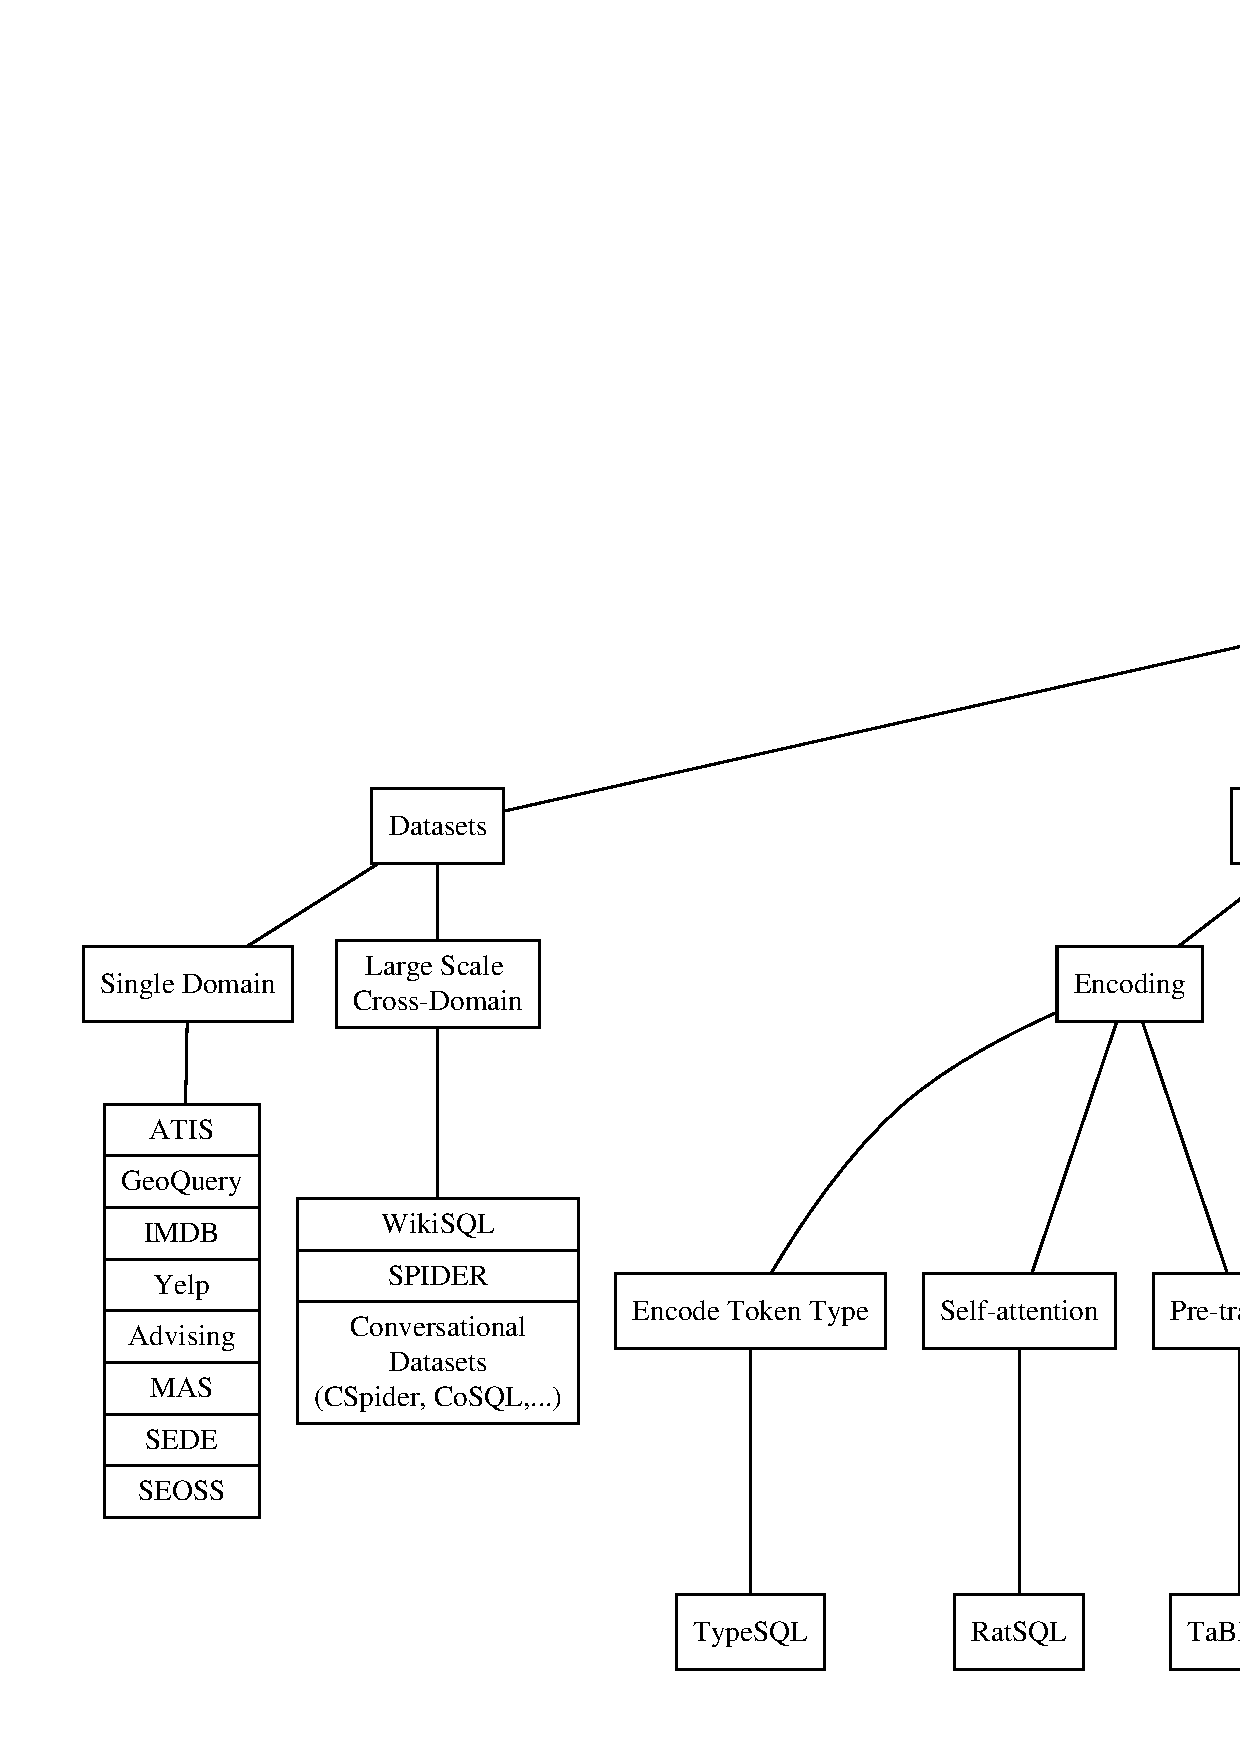
\includegraphics[width=1\linewidth]{pics/mindmap/mind}
    \caption{Text-to-SQL state-of-the-art Topology}
    \label{fig:mindmap}
\end{sidewaysfigure}

\subsection{Challenges}

Text-to-SQL is an intricate task, given the complexity and diversity of natural language and the structure and regulations of SQL. One of the most challenging aspects is to decipher the intent and significance of the natural language input, as it can be ambiguous or have varied interpretations. This can result in mistakes when building the corresponding SQL query, like selecting the incorrect table or columns or not recognizing the conditions for filtering or sorting the data. Additionally, the natural language input may contain typos or unknown words, which can complicate the mapping process. Moreover, the query generated may not be in the optimal form, as it has to take into account the various data types, operations, and constraints of the underlying database. Therefore, it is crucial to develop models and algorithms that can accurately map natural language to SQL queries.

Another challenge is dealing with the diverse and dynamic nature of databases, as the schema and data may change over time, and there may be variations in naming conventions and conventions across different databases. This can make it difficult for the model to correctly map the natural language input to the appropriate SQL elements, such as table and column names, and to handle variations in the structure of the SQL queries generated. Additionally, many real-world scenarios require integration with external knowledge bases and ontologies, which can be challenging to handle, especially when the external knowledge needs to be completed or consistent. Furthermore, the system must be robust to different types of user input, such as colloquial or informal language or input that needs to be completed or clarified. Additionally, Text-to-SQL systems must be able to handle errors in the input, such as typos, as well as rare edge cases that may not have been encountered during the training process. Finally, Text-to-SQL systems must be robust to the presence of out-of-vocabulary words and rare edge cases, which can be challenging to handle without significant amounts of labeled data, as well as the need to make accurate predictions with limited training data.

\clearpage
\subsection{Thesis Outline}

In this section, we provide an outline of our thesis.

\begin{itemize}
    \item Chapter 1 of the thesis provides an introduction to the topic of Text-to-SQL and discusses the challenges and contributions of the research.
    \item Chapter 2 provides technical background on Text-to-SQL, including early approaches, recent approaches, and important terminologies such as LSTM, encoder, decoder, transformers, BERT, semantic parsing, baseline model and incremental decoding.
    \item Chapter 3 describes the benchmark datasets used for evaluating Text-to-SQL methods, including the ATIS, GeoQuery, IMDb, Advising, WikiSQL, and Spider datasets.
    \item Chapter 4 presents an overview of SOAT Text-to-SQL solutions, including Seq2SQL, SQLNet, SyntaxSQLNet, IRNet, EditSQL, RAT-SQL, BRIDGE, and PICARD.
    \item Chapter 5 explains the evaluation metrics used to assess the performance of Text-to-SQL systems, including exact string matching, exact set matching, and distilled test suites.
    \item Chapter 6 presents an experiment and case study using the SEOSS dataset and the T5 PICARD model, with a focus on the metrics and evaluation results. The thesis also includes a section on EZ-PICARD and its Microservices practices.
    \item Chapter 7 concludes the thesis by summarizing the findings and exploring emerging challenges such as conversational Text-to-SQL.
\end{itemize}

\section{Technical Background}

In this chapter, we provide background information about the technical concepts related to the main topics of this thesis, which focus on natural language understanding and text generation. We focus on early and recent approaches and the terminology needed to understand the basics of this thesis.

The text-to-SQL problem, or \ac{NL2SQL}, is the following: Given a Natural Language Query (NLQ) on a \ac{RDB}, produce a SQL query equivalent to the \ac{NLQ}. It has been a holy grail for the database community for over 30 years to translate user queries into SQL. Several challenges include ambiguity, schema linking, vocabulary gaps, and user errors.

Early approaches to Text-to-SQL relied on rule-based and template-based methods, while recent approaches use neural networks and machine learning techniques. This allows them to handle a wide range of natural language inputs and generate more accurate SQL queries, which we will discuss further.

\subsection{Early Approaches}
Early approaches to Text-to-SQL focused on rule-based methods and template-based methods. These approaches relied on predefined templates and a set of predefined rules to generate SQL queries. These methods were based on the idea that a fixed set of templates and rules could be used to generate SQL queries for a wide range of natural language inputs. However, these methods were limited by their reliance on predefined templates and were not able to handle a wide range of natural language inputs.

\subsubsection{Rule-based methods}
In the case of rule-based methods, a set of predefined rules were used to map the natural language input to the corresponding SQL query. These rules were based on predefined grammar and were used to identify the SQL constructs present in the input text. These methods were able to generate simple SQL queries, but they were not able to handle more complex queries or handle variations in natural language inputs.

Early research in Text-to-SQL includes work by researchers such as Warren and Pereira in 1982\cite{Warren1982AnEE}, who proposed a rule-based method for generating SQL queries from natural language text. Their system used a set of predefined rules to map natural language constructs to SQL constructs and was able to generate simple SQL queries. Another example of a rule-based method is the work by Zelle and Mooney in 1996, who proposed CHILL parser\cite{Zelle1996LearningTP}, a system that used a predefined grammar to identify the SQL constructs present in the input text and generate the corresponding SQL query.

\subsubsection{Template-based methods}
Template-based methods, on the other hand, relied on predefined templates to generate SQL queries. These templates were based on a predefined set of SQL constructs and were used to map the natural language input to the corresponding SQL query. These methods were able to handle a limited set of natural language inputs, but they were not able to handle variations in the input or generate more complex queries. One of the very first systems that used predefined templates to map natural language inputs to SQL queries was able to handle a limited set of natural language inputs.

In summary, early approaches to Text-to-SQL were limited by their reliance on predefined templates and rules, which made them unable to handle a wide range of natural language inputs and generate complex SQL queries. The rule-based and template-based methods were two of the most common early approaches used in Text-to-SQL, each with their own strengths and limitations.
\subsection{Terminology}

Here is an updated list of key terminology and vocabulary that you may need to know before studying Text-to-SQL language models:

% \subsubsection{SQL (Structured Query Language)} The standard, a widely used programming language designed to manage relational databases, enables users to store, retrieve and manipulate data.
% \subsubsection{Natural Language Processing (NLP)}
% The field of study focuses on the interaction between human language and computers, which ranges from understanding spoken language to generating natural language text.

\subsubsection{Pre-training and Fine-tuning}

Pre-training refers to training a model on a large dataset and then fine-tuning it on a smaller dataset for a specific task, which helps to improve the model's performance on the specific task.

\subsubsection{SQL Constructs}

The elements of SQL language such as SELECT, FROM, WHERE, JOIN, are used to build queries and retrieve data from a database.

% \subsubsection{Evaluation Metrics}

% Measures used to evaluate the performance of Text-to-SQL models, such as accuracy, F1-score, and Exact Match score, compare different models and determine the best-performing model.

\subsubsection{Baseline Model}

A model that serves as a reference point or starting point for comparison, providing a baseline for performance against which other models can be evaluated.


% \subsubsection{Encoder-Decoder Architecture}

% A robust neural network architecture that utilizes an encoder\cite{cho-etal-2014-learning} to transform the input data into a compact and meaningful representation and a decoder to generate the desired output from that representation. This architecture has been widely utilized in many applications, such as language translation, image captioning, and text summarization, to produce high-quality results. Furthermore, the encoder-decoder architecture has the advantage of learning complex relationships between input and output, making it a suitable tool for many challenging tasks\cite{kumar2022deep}.


\subsubsection{Self-attention}

Self-attention \cite{https://doi.org/10.48550/arxiv.1706.03762} is a mechanism used in the transformer architecture that allows the model to determine the significance of various components of the input sequence to be able to generate an outcome that is more precise and sufficient. This mechanism allows the model to consider the relationships between different parts of the input sequence and to factor those relationships into its output. Further, self-attention lets the model capture patterns from the input sequence and use those patterns to generate more meaningful output. It is this combination of factors that makes self-attention such an essential tool for deep learning models.

\subsubsection{Incremental decoding}

A decoding strategy where the model generates a sequence of tokens one at a time, at each step conditioned on the previous tokens, the input, and the context of the sentence. This approach allows for a more dynamic and flexible generation of output, as it takes into account a variety of factors when making decisions about the next token. This strategy also helps the model avoid repeating itself, providing more diverse and unique outputs. Furthermore, incremental decoding helps the model to capture the nuance of the language better as it is able to build upon previous decisions and refine its output as it progresses\cite{huang-mi-2010-efficient}.

\subsubsection{Semantic parsing}

Semantic parsing\cite{krishnamurthy-etal-2017-neural} is an area of natural language processing that involves extracting the meaning or intent from text. One class of Semantic Parsing, Text-to-SQL, involves converting natural language problems into SQL query statements. This is a challenging task, one that requires the use of advanced machine learning and natural language processing algorithms. As such, the research conducted in this field seeks to explore the various solutions and practices employed by researchers to tackle this problem effectively. Furthermore, it is also important to note that this problem is not just limited to converting natural language into SQL query statements, as other applications of Semantic Parsing have been explored, such as \ac{NLG}. Overall, by understanding the various techniques used for Semantic Parsing, we can better understand the complexities involved in this task and how best to approach it.


\subsection{Text Processing}

In this section, we will discuss the fundamental elements of the text processing pipeline in natural language processing (NLP) tasks. The pipeline involves several steps, including tokenization, embedding, prediction, and conversion of embeddings back to words. These elements work together to transform raw text into a suitable format for NLP models and generate human-readable output.

\subsubsection{Tokenization}

Tokenization is a fundamental process in natural language processing (NLP) that involves breaking the raw text into individual words, phrases, or other meaningful units called tokens. This step is essential for preparing the text for further processing, as it enables the model to analyze and understand the text at a more granular level, thus simplifying the analysis and processing of the content.
Various tokenization methods can be employed, including rule-based, statistical, and more advanced approaches like subword tokenization and Byte Pair Encoding (BPE). Rule-based methods often use pre-defined rules to separate words, phrases, or sentences, while statistical methods rely on the frequency and distribution of words and characters in the text.
Subword tokenization and Byte Pair Encoding (BPE) are advanced techniques that account for the morphological structure of words, generating tokens based on common subword units. This approach is beneficial for handling out-of-vocabulary words and capturing meaningful information from rare or previously unseen words.
In addition to word-level tokenization, other techniques exist, such as subword-level and character-level tokenization. Subword-level tokenization further divides words into smaller subword units, which can capture more linguistic information and improve the model's ability to handle morphologically rich languages. On the other hand, character-level tokenization breaks text into individual characters, providing even more granularity and enabling the model to learn character-level patterns.

\subsubsection{Embeddings}

WordPiece embeddings\cite{DBLP:journals/corr/WuSCLNMKCGMKSJL16} is a tokenization approach used in natural language processing (NLP) to break down words into smaller units, also known as pieces. It is an extension of the original word2vec parameter learning algorithm and is used to address out-of-vocabulary (OOV) words, which are words that did not appear in the training data.
This technique divides each word into a series of subword units learned during the training phase based on their frequency and consistency within words. These subword units are stored in a shared vocabulary, dubbed the WordPiece vocabulary, and can be used for multiple words.
This system can represent rare or unseen words as a combination of more common subword units, which are more likely to be in the vocabulary. As a result, the model can handle OOV words more efficiently and reduce the vocabulary size, leading to a more economical representation of the language.
In NLP models, words are usually portrayed as dense vectors referred to as word embeddings. WordPiece embeddings extend this representation by breaking words down into subword units and representing each piece as a dense vector. These subword embeddings are then combined to represent the whole word.
The use of WordPiece embeddings has various advantages in NLP models. Firstly, it enables the model to treat OOV words more effectively by representing them as a combination of more common subword units. Secondly, it decreases the vocabulary size, resulting in a more succinct representation of the language. Finally, it enhances the model's capability to learn fine-grained representations of words and their meanings, resulting in improved performance in NLP tasks.

\subsubsubsection{Word2Vec}

Word2Vec\cite{DBLP:journals/corr/Rong14} is a well-known word embedding approach in NLP that encodes words as dense vectors in an unending, high-dimensional area. This technique is designed to capture the significance and context of words, providing an improved representation of words compared to classic one-hot encoding.
The fundamental concept behind Word2Vec is to train a neural network to anticipate the context words about a target word, given the target word. As the model is trained, the weights of the neural network are adjusted in such a way that the dot product of the input layer (representing the target word) and the output layer (representing the context words) closely estimate the probability distribution of the context words given the target word.
Word2Vec can be trained to employ two different algorithms: Continuous Bag-of-Words (CBOW) and Skip-gram. CBOW predicts the target word given the context words, while Skip-gram predicts the context words given the target word. The algorithm selection relies on the particular NLP task and the data available for training.

\subsubsubsection{\ac{GloVe}}

Global Vectors for Word Representation, developed by Pennington et al.\cite{pennington-etal-2014-glove}, is another popular embedding technique. GloVe combines the advantages of both global matrix factorization methods and local context window methods. It learns embeddings by considering the co-occurrence probabilities of words within a corpus, thus capturing the global corpus statistics. GloVe embeddings demonstrate better performance on various NLP tasks, such as semantic similarity and analogy detection, compared to Word2Vec.

\subsubsubsection{\ac{ELMo}}

Embeddings from Language Models, introduced by Peters et al.\cite{ELMo}, is a more advanced approach that generates contextualized word embeddings. Unlike Word2Vec and GloVe, which produce static embeddings for each word, ELMo generates embeddings that are context-dependent. ELMo is based on a bidirectional LSTM language model, which learns different layers of representations for each word, capturing both low-level syntactic features and high-level semantic features. The contextualized nature of ELMo embeddings has proven to significantly improve performance in various downstream NLP tasks.

\subsubsection{Prediction}

Prediction is a critical step in many NLP tasks, such as text classification, named entity recognition, and machine translation. In this step, models utilize embeddings to make predictions or generate output based on the input text. Various techniques can be employed for prediction, including feedforward neural networks, recurrent neural networks (RNNs), long short-term memory (LSTM) networks, gated recurrent units (GRUs), and transformer-based models.

\subsubsubsection{\ac{LSTM}}

A type of recurrent neural network designed to store information over a more extended period than traditional neural networks, allowing it to capture long-term dependencies better \cite{Hochreiter1997LongSM}.
This makes it especially well-suited for tasks such as language modeling and text generation, where it can take into account the context of the text in order to generate more accurate outputs.
In addition, LSTM networks can identify patterns in the data that would be difficult for traditional networks to capture. This makes them ideal for tasks such as sequence prediction and classification, where they can identify patterns that would otherwise be too subtle for traditional networks to detect.

\subsubsection{Conversion of Embeddings Back to Words}

The final step in the text processing pipeline is converting the embeddings back into human-readable text. This process is typically part of the decoding phase in sequence-to-sequence models, where the model takes the embeddings and generates a sequence of words in the target language or format. Several decoding strategies can be used to achieve this, such as greedy search, beam search, and sampling methods like top-K sampling and nucleus sampling. We will discuss these strategies in more detail in the next section.
The architecture introduced in the paper "Attention Is All You Need" by Vaswani et al. in 2017\cite{https://doi.org/10.48550/arxiv.1706.03762}, known as Transformers, is a revolutionary breakthrough in the way sequences of data are processed. By utilizing self-attention mechanisms, the model is able to achieve improved efficiency and accuracy, while also being much simpler to implement and deploy. This makes it particularly appealing for a wide range of applications, from natural language processing to computer vision. Furthermore, due to their scalability, Transformers are able to accommodate large data sets, enabling them to be used to tackle more complex tasks. As such, Transformers are becoming increasingly popular in the field of machine learning and artificial intelligence, with more and more research being done to further explore its capabilities.

There were many excellent works around 2015 on learning word vectors to continuous representations for words where the identity of a word was mapped to a fixed-length vector which ideally encoded some meaning about the word in a continuous space and for a long time.

That has been an essential part of the NLP pipeline, especially for deep learning models where these pre-trained word vectors were used, typically trained using an unsupervised objective, and new models were fed and trained on top of them.

An important paper in 2017 that helped researchers change their way of thinking towards the transfer learning paradigm was the unsupervised sentiment neuron paper from people at OpenAI \cite{DBLP:journals/corr/RadfordJS17}, which essentially showed that by just training a language model on a purely unsupervised objective, the model could learn concepts that were potentially useful for downstream tasks.

In 2018, the NLP community had a couple of super important papers, \\
including the ULMFiT\cite{ELMo}, which took the recipe from semi-supervised sequence learning, added some tweaks, figured out how to get it working better, and got some noble results with a similar pipeline, pre-training a language model, fine-tuning on a downstream task.

And then, ELMo\cite{ELMo} showed that we could get significantly better performance by using a bi-directional language model.

Then GPT1 \cite{Radford2018ImprovingLU} came along, saying that instead of using analyst TM, we can get good performance by using a transformer with a language model.

Finally, in 2018, BERT \cite{devlin-etal-2019-bert} showed that a bi-directional transformer could get outstanding performance, and by the end of 2018, many researchers were convinced that this was the path forward given all of the impressive results that these papers and a few others showed.

Following these researches, there has been a burst of work on transfer learning for NLP, working on various methods, different pre-training ideas, datasets, and different benchmark tasks.

In Google T5, it is tried to use all the new studies in transfer learning and combine the best selection of these studies to achieve state-of-the-art results on many benchmarks covering summarization, classification, question answering, and more.
\subsection{Learning Techniques}

The advancement of Text-to-SQL research has been driven by various learning techniques that address specific challenges in the field. We provide a comprehensive overview of these learning techniques, focusing on both fully supervised and weakly supervised methods.

\subsubsection{Fully Supervised Learning Techniques}

Fully supervised learning approaches depend on labeled data to train models. We explore various cutting-edge methods proposed to enhance Text-to-SQL generation.

\subsubsection*{Active Learning}

Active learning aims to reduce the labeled data needed for training by selectively identifying the most informative examples. Ni et al.\cite{ni2019merging} developed an active learning framework that uses uncertainty estimation to pinpoint samples that would gain the most from human annotations.

\subsubsection*{Interactive/Imitation Learning}

Interactive or imitation learning concentrates on learning from demonstrations, with a model trying to replicate expert behavior. Yao et al. \cite{yao-etal-2019-model} presented an interactive learning method that integrates user feedback to improve the model's comprehension of intricate SQL queries.

\subsubsection*{Multi-task Learning}

Multi-task learning consists of training a single model on multiple related tasks concurrently. Chang et al. \cite{chen2021leveraging} investigated a multi-task learning framework for Text-to-SQL generation, illustrating that sharing information across tasks can result in enhanced performance.

\subsubsection{Weakly Supervised Learning Techniques}

Weakly supervised learning approaches employ weak or noisy labels for training, often diminishing the need for extensive human annotation.

\subsubsection*{Reinforcement Learning}

Reinforcement learning focuses on learning through trial and error, with models receiving feedback via rewards or penalties. Seq2SQL Zhong et al. \cite{zhong_seq2sql_2017} applied reinforcement learning to Text-to-SQL generation, demonstrating that such a method can effectively learn from weak supervision, for instance, it allowed Seq2SQL to understand different orders of WHERE clauses in a query.

\subsubsection*{Meta-learning and Bayesian Optimization}

Meta-learning entails training models to learn how to learn effectively. Huang et al. \cite{huang-etal-2018-natural} suggested a meta-learning strategy for Text-to-SQL tasks, enabling the model to swiftly adapt to new tasks or domains with limited labeled data.

Agarwal et al. \cite{pmlr-v97-agarwal19e} combined meta-learning and Bayesian optimization for weakly supervised Text-to-SQL tasks. This technique enables models to adapt more efficiently to new tasks while taking advantage of limited supervision, ultimately reducing the necessity for large amounts of labeled data.
\subsection{Recent Approaches}

Recent approaches to Text-to-SQL have focused on using neural networks and machine learning techniques to generate SQL queries. These methods use large amounts of training data to learn the relationship between natural language and SQL and can generate SQL queries for a wide range of inputs. These methods can handle a wide range of natural language inputs and are not limited by predefined templates or rules. Additionally, recent approaches leverage pre-trained models such as \ac{BERT} \cite{devlin-etal-2019-bert}, GPT-2 \cite{radford2019language}, and T5 \cite{raffel_exploring_2020}, which have been pre-trained on a large corpus of text, to fine-tune text-to-SQL tasks, which enables them to understand the natural language inputs better and generate more accurate SQL queries.

One favored strategy is using encoder-decoder architecture, which uses an encoder to encode the natural language input and a decoder to generate the corresponding SQL query. The encoder is a pre-trained language model such as BERT, which is fine-tuned on the task of text-to-SQL, and the decoder is a neural network that generates the SQL query. This architecture effectively generates accurate SQL queries for various natural language inputs.

Another recent approach is using reinforcement learning to generate SQL queries, where a neural network generates a sequence of SQL tokens and is trained using a reward signal based on the quality of the generated query. This approach is adequate for generating more complex SQL queries and handling variations in natural language inputs.

In recent years, the Transformer architecture has significantly impacted natural language processing and machine learning, including in the field of Text-to-SQL. The Transformer architecture, presented in the paper "Attention Is All You Need" by Vaswani in 2017 \cite{https://doi.org/10.48550/arxiv.1706.03762}, is a neural network architecture that uses self-attention mechanisms to process data sequences, such as natural language text.

% One of the key advantages of the Transformer architecture is its ability to handle long-term dependencies in data sequences, making it well-suited for tasks such as natural language understanding and text generation. This has led to the development of pre-trained Transformer models, such as BERT, GPT-2, and T5, that have been trained on a large corpus of text and can be fine-tuned on specific tasks such as Text-to-SQL.

The use of pre-trained Transformer models such as BERT in Text-to-SQL has shown to be effective in improving the performance of the models. The pre-trained models have a good understanding of the natural language, which enables them to understand the input text better and generate more accurate SQL queries.
The Transformer architecture and pre-trained models such as BERT have significantly impacted recent studies in the field of Text-to-SQL. The ability of the Transformer architecture to handle long-term dependencies in sequences of data and the pre-trained models' good understanding of natural language has made it possible to generate more accurate SQL queries for a wide range of natural language inputs.

In outline, recent approaches in Text-to-SQL leverage neural networks and machine learning techniques, such as encoder-decoder architecture and reinforcement learning. These approaches use large amounts of training data and pre-trained models such as BERT to generate accurate SQL queries for a wide range of natural language inputs.
\section{Benchmark Dataset}

\begin{figure}[htb]
    \centering
    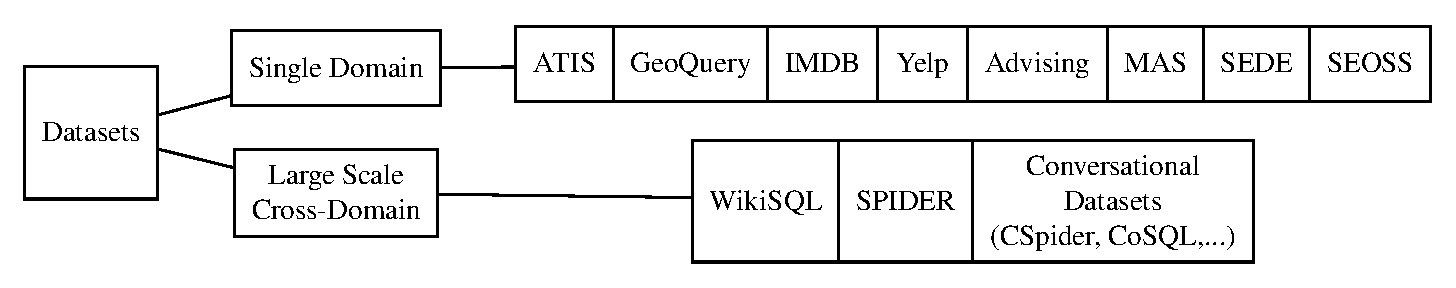
\includegraphics[width=0.6\textwidth]{pics/mindmap/ds/ds.eps}
    \label{fig:ds}
\end{figure}

Datasets are crucial in developing and evaluating Text-to-SQL models for semantic parsing of natural language phrases. Various benchmark datasets are available, each with unique characteristics and features. Examples of early datasets include ATIS\cite{dahl-etal-1994-expanding}, GeoQuery\cite{10.1007/3-540-44795-4_40}, and Yelp\cite{10.1145/3133887}, which focus on a single topic and database. More recent datasets, such as WikiSQL\cite{zhong_seq2sql_2017} and Spider\cite{yu_spider_2019}, are larger and cover a broader range of domains.

These benchmark datasets provide a standardized testbed for evaluating the performance of Text-to-SQL models and are widely used in the research community. They vary in complexity, size, and annotation, allowing researchers to evaluate models' performance at different levels and scenarios. Additionally, new datasets include more advanced queries to assess the generalization capabilities of models. This chapter will review the complete benchmark datasets used in the Text-to-SQL Semantic Parsing community and discuss their significance for the research community.

\subsection{Single-Domain}

\subsubsection{ATIS (Air Travel Information System) and GeoQuery}
\label{sec:atis}

ATIS (Air Travel Information System)\cite{dahl-etal-1994-expanding} and GeoQuery \cite{10.1007/3-540-44795-4_40} are two datasets that are frequently utilized for semantic parsing, a technique for converting natural language inquiries into a structured meaning representation. The ATIS dataset consists of audio recordings and hand transcripts of individuals using automated travel inquiry systems to search for information regarding flights. It is structured using a relational schema to organize data from the official airline guide, with 25 tables containing information concerning fares, airlines, flights, cities, airports, and ground services.
All questions concerning this dataset can be answered using a single relational query. This makes it an ideal choice for training deep learning models, as it is designed for a specific domain and the queries are relatively straightforward.

Furthermore, the questions in the ATIS dataset \cite{dahl-etal-1994-expanding} are mainly limited to select and project queries. On the other hand, GeoQuery \cite{10.1007/3-540-44795-4_40} is made up of seven tables from the US geography database and 880 natural languages to SQL pairings. It includes geographic and topographical characteristics such as capitals, populations, and landforms. While both datasets are regularly employed to train deep learning models, GeoQuery \cite{10.1007/3-540-44795-4_40} is more comprehensive and provides a wider range of queries than ATIS. This includes JOIN and nested queries, as well as grouping and order queries, which are absent in the ATIS dataset\cite{dahl-etal-1994-expanding}. As a result, GeoQuery is better equipped to answer more complex queries, making it a better choice for training AI models.

% A relational schema is used to organize data from the official airline guide in the ATIS corpus. There are 25 tables containing information about fares, airlines, flights, cities, airports, and ground services. All questions related to this dataset can be answered using a single relational query. The relational database uses shorter tables for this dataset to answer queries intuitively.

% Here is an example query from the ATIS dataset: Input is in natural language, and the output is in \lambda calculus.

% \begin{figure}[htb]
%     \centering
%     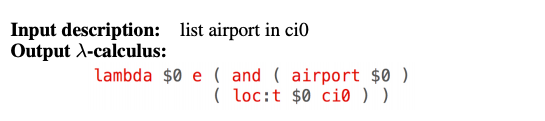
\includegraphics[width=0.8\textwidth]{pics/db/ATIS.png}
%     \caption{Example from ATIS dataset for semantic parsing}
%     \label{fig:ATIS}
% \end{figure}

% \subsubsection{GeoQuery Dataset}

% United States geography is represented in the Geoquery dataset. About 800 facts are expressed in Prolog. State, city, river, and mountain information can be found in the database. Geographic and topographical attributes such as capitals and populations make up the majority of the attributes.

\begin{table}[htbp]
    \centering
    \caption{Example of a complex ATIS SQL query}
    \label{tab:ATISsqlquery}
    \begin{tabular}{|l|p{10cm}|}
        \hline
        Text & I would like a flight between BOSTON and ATLANTA on any day at one in the afternoon.                                                                                                                                                                                                                                                                                                                                                                                                                                    \\ \hline
        SQL  & \small\texttt{SELECT DISTINCT flight.FLIGHT\_ID FROM AIRPORT\_SERVICE AS airport\_service , AIRPORT\_SERVICE AS airport\_service2 , CITY AS city2 , CITY AS city , FLIGHT AS flight WHERE ( city.CITY\_CODE = airport\_service2.CITY\_CODE AND city.CITY\_NAME = "ATLANTA" AND flight.DEPARTURE\_TIME = 1300 AND flight.TO\_AIRPORT = airport\_service2.AIRPORT\_CODE ) AND city2.CITY\_CODE = airport\_service.CITY\_CODE AND city2.CITY\_NAME = "BOSTON" AND flight.FROM\_AIRPORT = airport\_service.AIRPORT\_CODE ;} \\ \hline
    \end{tabular}
\end{table}

\subsubsection{IMDb Dataset}

The IMDb dataset is a well-known dataset in the machine learning community. It contains 50,000 reviews from IMDb and has a limit of 30 reviews per movie\cite{maas-EtAl:2011:ACL-HLT2011}. It is noteworthy that the dataset is balanced in terms of positive and negative reviews, which are equally represented. When creating the dataset, reviews with a score of 4 out of 10 were considered negative and those with a score of 7 out of 10 were considered positive. Neural reviews were excluded to maintain the quality of the dataset. The dataset is divided into training and testing datasets, each with an equal portion. To ensure fairness and accuracy in the results, the dataset creators have taken special care to keep the training and testing datasets balanced.

% \begin{figure}[H]
%     \centering
%     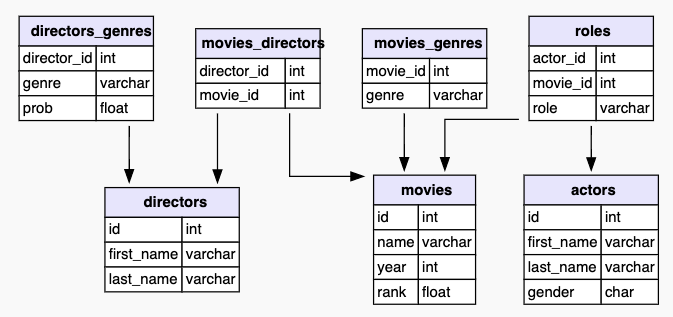
\includegraphics[width=0.8\textwidth]{pics/db/IMDb.png}
%     \caption{Database Structure of IMDb dataset\cite{dahl-etal-1994-expanding}}
%     \label{fig:IMDb}
% \end{figure}

\begin{figure}[H]
    \label{tab:IMDBsqlquery}
    \begin{AIbox}{Example of a complex IMDb SQL query}
        \vspace{-5px}
        \parbox{1\textwidth}{\scriptsize
        \begin{alltt} 
            {\bf Utterance:} \\ 
            What year was the movie The Imitation Game produced?
            \\
            {\bf Query:} \\
            SELECT MOVIEalias0.RELEASE\_YEAR FROM MOVIE AS MOVIEalias0 WHERE MOVIEalias0.TITLE = 'The Imitation Game' ;
        \end{alltt}
        }
        \vspace{-5px}
    \end{AIbox}
\end{figure}

% \begin{table}[H]
%     \centering
%     \caption{Example of a complex IMDb SQL query}
%     \begin{tabular}{|l|p{10cm}|}
%         \hline
%         Utterance & What year was the movie The Imitation Game produced?                                                                       \\ \hline
%         Query  & \small\texttt{SELECT MOVIEalias0.RELEASE\_YEAR FROM MOVIE AS MOVIEalias0 WHERE MOVIEalias0.TITLE = 'The Imitation Game' ;} \\ \hline
%     \end{tabular}
% \end{table}

\subsubsection{Advising Dataset}

The Advising dataset\cite{finegan-dollak-etal-2018-improving} was created in order to propose improvements in Text-to-SQL systems. The creators of the dataset compare human-generated and automatically generated questions, citing properties of queries that relate to real-world applications. The dataset consists of questions from the University of Michigan students about courses that lead to particularly complex queries. The data is obtained from a fictional student database which includes student profile information such as recommended courses, grades, and previous courses. Moreover, in order to obtain the data for the dataset, academic advising meetings were conducted where students were asked to formulate questions they would ask if they knew the database. After obtaining the questions, the creators of the dataset compared the query results with those from other datasets such as ATIS [\ref{sec:atis}], GeoQuery, and Scholar. Many of the queries in the Advising dataset were the same as those found in the other datasets.

% \begin{figure}[htb]
%     \centering
%     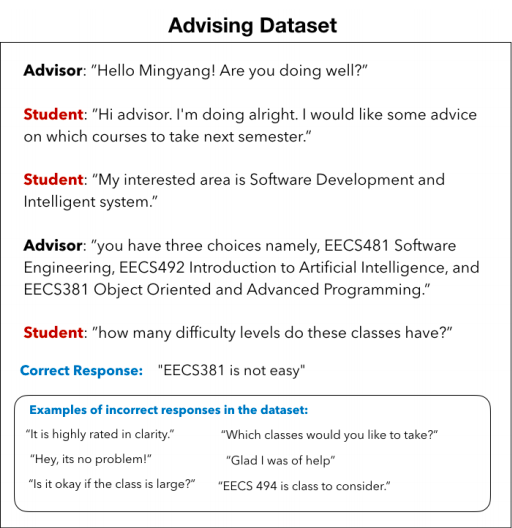
\includegraphics[width=0.5\textwidth]{pics/db/Advising.png}
%     \caption{Example from Advising dataset \cite{vig_comparison_2019}}
%     \label{fig:Advising}
% \end{figure}
\subsubsection{MAS (Microsoft Academic Search)}

MAS, or Microsoft Academic Search\cite{roy2013the}, is a database of academic and social networks and a collection of queries. It has a total of 17 tables in its database, as well as 196 natural languages to SQL pairs. MAS can handle join, grouping, and nested queries but does not support ordering queries.

There are a few limitations to be aware of when using natural language queries within MAS. Firstly, all-natural language questions must begin with the phrase ”return me” and can not include an interrogative statement or a collection of keywords. Additionally, all queries must follow the proper grammatical conventions.

\subsubsection{SEDE}

\ac{SEDE} \cite{DBLP:journals/corr/abs-2106-05006} is from a popular online question-and-answer platform with more than 3 million questions, and it recently released a benchmark dataset of SQL queries containing 29 tables and 211 columns. This dataset comprises real-world questions from the Stack Exchange website, such as published posts, comments, votes, tags, and awards.

Although these datasets contain a variety of real-world challenges, they still need to be more tricky to parse semantically due to the complexity of the questions they contain. After further analysis of the 12,023 questions asked on the platform, a total of 1,714 have been verified by humans, which makes it an ideal choice for training and validating the model. This benchmark dataset is highly valuable and helpful for research in natural language processing, as it provides an extensive list of real-world challenges that have rarely been seen in other semantic parsing datasets.

\begin{figure}[H]
    \label{fig:sede_sql}
    \begin{AIbox}{An example of a Complex SEDE utterance}
        \vspace{-5px}
        \parbox{1\textwidth}{\scriptsize
        \begin{alltt} \larger
            {\bf Utterance:} \\ 
            Check if Votes.CreationDate is always a date
            \\
            {\bf Query:} \\
            SELECT Name, Count(*)as [Count], DatePart(Hour, Votes.CreationDate)as [hour],DatePart(Minute, Votes.CreationDate)as [minute],DatePart(Second, Votes.CreationDate)as [second],DatePart(Millisecond, Votes.CreationDate)as [ms] FROM Votes JOIN VoteTypes ON VoteTypeId = VoteTypes.Id GROUP BY Name, DatePart(Hour, Votes.CreationDate),DatePart(Minute, Votes.CreationDate),DatePart(Second, Votes.CreationDate),DatePart(Millisecond, Votes.CreationDate)
        \end{alltt}
        }
        \vspace{-5px}
    \end{AIbox}
    
    \captionsetup{font={scriptsize,color=white}, skip=-20pt}
    \caption{An example of a Complex SEDE utterance}
\end{figure}
\subsubsection{SEOSS}

\ac{SEOSS} dataset is a compilation of natural language expressions with seven alternative phrasings, each linked to a single SQL query. In total, 166 questions (expressions) were organized. The natural language expressions were mainly obtained from existing literature and modified to match the data identified in the issue tracking system (ITS) and version control system (VCS) of an existing software project (namely Apache Pig). This data was extracted and saved into an SQLite database by Rath et al. \cite{RATH2019104005}.

\begin{figure}[H]
    \centering
    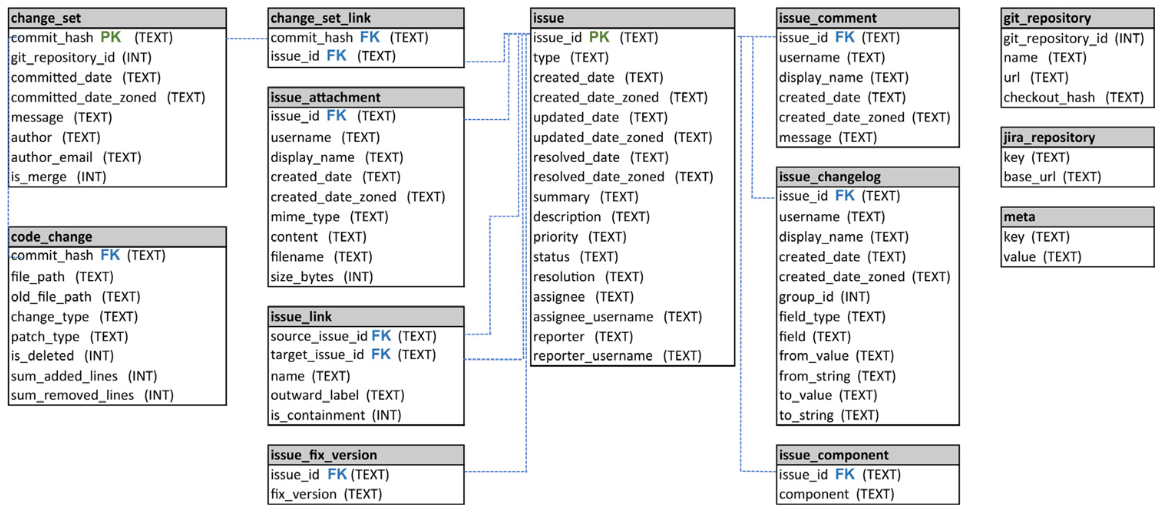
\includegraphics[width=1\textwidth]{pics/seoss/pig.png}
    \caption{Database Schema of the PIG Database \cite{TOMOVA2022108211}}
    \label{fig:SESS}
\end{figure}

Expressions are labeled into two different tags, development and research. Eighty-one queries with a focus on software needs of stakeholders and developers or from typical use cases' queries of issue tracking systems were labeled as 'development,' and 63 queries containing issue tracking systems information or version control systems were labeled as 'research.' Also, 22 records were generated from the content in questions stakeholders asked within the comment sections of issues of type bug, enhancement/improvement, new feature/feature request, and tasks of 33 open-source Apache projects, which were extracted and stored into databases by Rath and Mäder\cite{RATH2019104005}.
In SEOSS-Queries\cite{TOMOVA2022108211} research, they experienced RatSQL and SQLNet methods on the SEOSS dataset and released their evaluation steps. In this research, we will use the same dataset to evaluate state-of-the-art models currently available in the literature and used in SPIDER for this dataset.


% TODO: need more about the Hardness of the SEOSS dataset
% \begin{figure}[H]
%     \centering
%     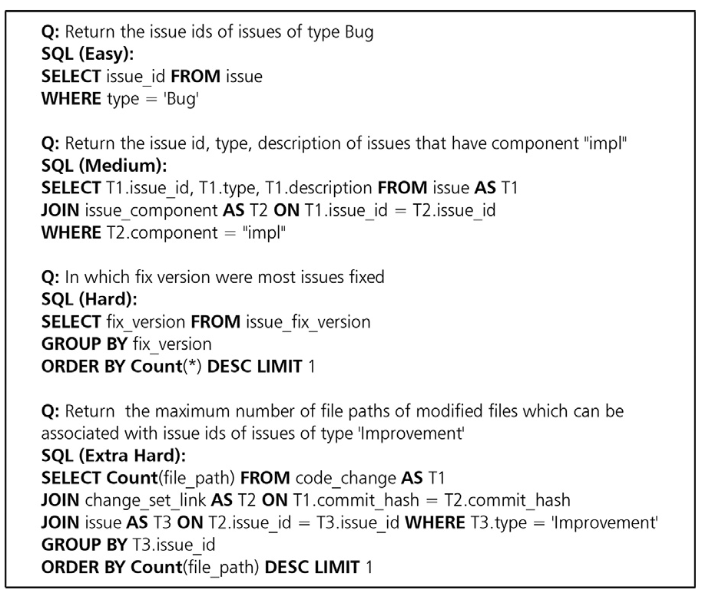
\includegraphics[width=0.8\textwidth]{pics/seoss/seoss.png}
%     \caption{\small Examples of queries with different levels of complexity in SEOSS-Queries \cite{TOMOVA2022108211}}
%     \label{fig:SESS2}
% \end{figure}

\begin{figure}[H]
    \label{fig:SESS2}
    \begin{AIbox}{An example of an extra-hard SEOSS record}
        \vspace{-5px}
        \parbox{1\textwidth}{\scriptsize
        \begin{alltt} \larger
            {\bf Utterance:} \\ 
            Return  the maximum number of file paths of modified files which can be associated with issue ids of issues of type 'Improvement
            \\
            {\bf Query:} \\
            SELECT Count(file\_path) FROM code\_change AS T1 JOIN change\_set\_link AS T2 ON T1.commit\_hash = T2.commit\_hash JOIN issue AS T3 ON T2.issue\_id = T3.issue\_id WHERE T3.type = 'Improvement' GROUP BY T3.issue\_id ORDER BY Count(file\_path) DESC LIMIT 1
        \end{alltt}
        }
        \vspace{-5px}
    \end{AIbox}
    
    \captionsetup{font={scriptsize,color=white}, skip=-20pt}
    \caption{An example of an extra-hard SEOSS record}
\end{figure}



\clearpage

\subsection{Large Scale Cross-Domain}

\subsubsection{WikiSQL}

WikiSQL consists of 80,654 natural language questions and corresponding SQL queries on 24,241 tables extracted from Wikipedia. Neither the train nor development sets contain the database in the test set. Databases and SQL queries have simplified the dataset's creators' assumptions. This dataset consists only of SQL labels covering a single SELECT column and aggregation and WHERE conditions. Furthermore, all the databases contain only one table.

The database does not include complex queries involving advanced operations like JOIN, GROUP BY, ORDER BY, etc. Prior to the release of SPIDER, this dataset was considered to be a benchmark dataset. Using WikiSQL has been the subject of a great deal of research. WikiSQL's "WHERE" clause has been recognized as one of the most challenging clauses to parse semantically, and SQLNet and SyntaxSQL were previous state-of-the-art models.


\begin{figure}[htb]
    \centering
    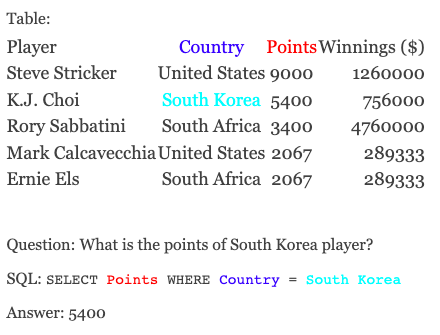
\includegraphics[width=0.5\textwidth]{pics/db/WikiSQL.png}
    \caption{Example from WikiSQL dataset\cite{DBLP:journals/corr/abs-1902-01069}}
    \label{fig:WikiSQL}
\end{figure}

The WikiSQL challenge is a research competition focused on developing natural language interfaces for databases. The challenge includes several state-of-the-art Text-to-SQL solutions proposed by different research teams.

One example of a state-of-the-art Text-to-SQL solution in the WikiSQL challenge is the Seq2SQL model, which uses a sequence-to-sequence learning framework to map natural language input to SQL queries. The model uses an attention mechanism to align the input and output sequences and a pointer network to handle SQL queries with complex structural dependencies.

Another example is the Spider model, which uses a combination of recurrent and convolutional neural networks to learn the mapping between natural language and SQL queries. The model uses a hierarchical structure to process the natural language input, with separate modules for understanding the query's intent, columns, and constraints.
One difference between these research approaches is the specific deep learning architecture used. The Seq2SQL model uses a sequence-to-sequence framework, while the Spider model uses a combination of RNNs and convolutional neural networks. Additionally, the Spider model uses a hierarchical structure to process the natural language input, while the Seq2SQL model processes the input linearly.

Another difference is in the evaluation metrics used. The Seq2SQL model is evaluated using the execution accuracy of the generated SQL queries, while the Spider model is evaluated using a combination of execution accuracy and natural language understanding metrics.
Overall, both the Seq2SQL and Spider models are state-of-the-art Text-to-SQL solutions that have achieved high performance in the WikiSQL challenge. However, their specific architectures and evaluation metrics differ, which can affect their performance and accuracy on different tasks.
\subsubsection{SPIDER}

The SPIDER database contains 10K questions and 5K+ complex SQL queries covering 138 different domains across 200 databases. As opposed to previous datasets (most of which used only one database), this one incorporates multiple datasets. Creating this dataset took 11 Yale University students, 1,000 man-hours in total.

Spider contains queries with a lot of intricate SQL elements. In comparison to the sum of the previous Text-to-SQL datasets, Spider comprises around twice as many nested queries and ten times as many ORDER BY (LIMIT) and GROUP BY (HAVING) components.

Creating this corpus was primarily motivated by the desire to tackle complex queries and generalize across databases without requiring multiple interactions.

\begin{figure}[htb]
    \centering
    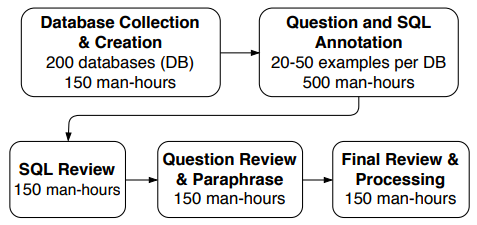
\includegraphics[width=0.6\textwidth]{pics/db/Spider.png}
    \caption{Process of creating SPIDER dataset\cite{yu_spider_2019}}
    \label{fig:Spider}
\end{figure}

Creating a dataset involves three main aspects: SQL pattern coverage, SQL consistency, and question clarity. Several databases from WikiSQL are included in the dataset. The table is complex as it links several tables with foreign keys. In SPIDER, SQL queries include: SELECT with multiple columns and aggregations, WHERE, GROUP BY, HAVING, ORDER BY, LIMIT, JOIN, INTERSECT, EXCEPT, UNION, NOT IN, OR, AND, EXISTS, LIKE.

The complexity of the dataset increases and the accuracy of solutions drops as the number of foreign keys in the database increases. This is mainly due to the difficulty in selecting the relevant column and table names from a complex database schema. Furthermore, complex database schemas present a major challenge for the model to accurately capture the relationship between different tables which involve foreign keys. SQL queries with a higher number of foreign keys tend to join more tables, suggesting a need for more effective methods to encode the connection between tables with foreign keys.

\subsubsection*{SQL Hardness Criteria}

In order to gain a better understanding of how the model performs on different queries, we have divided SQL queries into four difficulty levels: easy, medium, hard, and extra hard. This classification is based on the number of SQL components, selections, and conditions. Queries that contain multiple SQL keywords (e.g., GROUP BY, ORDER BY, INTERSECT, nested subqueries, column selections, aggregators) are generally considered more complex. For example, a query is considered hard if it includes more than two SELECT columns, more than two WHERE conditions, and GROUP BY two columns, or contains EXCEPT or nested queries. If it contains even more additions on top of that, it is considered extra hard.

\begin{figure}[htb]
    \centering
    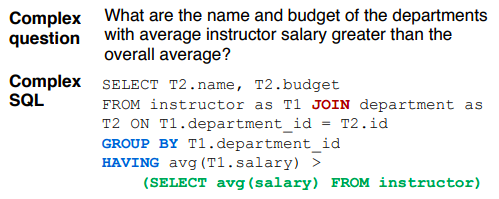
\includegraphics[width=0.8\textwidth]{pics/db/Spider2.png}
    \caption{Example of Question-Query set from SPIDER\cite{yu_spider_2019}}
    \label{fig:Spider2}
\end{figure}


SPIDER's exact matching accuracy\ref{eval} was 12.4\% compared to existing state-of-the-art models. As a result of its low accuracy, SPIDER presents a strong research challenge. Current SPIDER accuracy is above 75.5\% with an exact set match without values (refers to values in the WHERE clause) and above 72.6\% with values using PICARD\ref{picard}.

The SPIDER challenge is a research competition dedicated to developing cutting-edge Text-to-SQL and Semantic Parsing solutions. In this challenge, participants strive to develop algorithms that can automatically generate structured SQL queries from natural language input, to improve the performance and accuracy of Text-to-SQL models.

In this challenge, numerous state-of-the-art Text-to-SQL solutions have been proposed, such as the Spider model. This model uses a combination of recurrent and convolutional neural networks to learn the mapping between natural language and SQL queries. This model also has a hierarchical structure, which allows it to process the natural language input more effectively, thereby allowing it to handle complex queries and variations in language with greater precision and accuracy. This model successfully generates accurate and efficient SQL queries from natural language inputs.

One difference between the SPIDER and WikiSQL challenges is the specific dataset that is used for evaluation. The SPIDER challenge uses a dataset of complex SQL queries and natural language questions derived from real-world databases, while the WikiSQL challenge uses a dataset of more straightforward SQL queries and natural language questions derived from Wikipedia articles. This difference in the dataset can affect the performance and accuracy of the models on the different tasks.

Another difference is in the evaluation metrics used. The SPIDER challenge evaluates the models using execution accuracy and natural language understanding metrics, while the WikiSQL challenge evaluates the models using only execution accuracy. This difference in the evaluation metrics can affect how the models are trained and their performance on the tasks. We will discuss the evaluation metrics used in the SPIDER challenge in more detail in the next section\ref{eval}.
\subsubsection{Multi-Lingual Large Scale Datasets}

In this study, we are only focusing on English datasets. Nevertheless, Researchers have produced several large-scale text-to-SQL datasets in diverse languages, such as CSpider\cite{min-etal-2019-pilot}, TableQA Sun et al. \cite{DBLP:journals/corr/abs-2006-06434}, DuSQL Wang et al. (2020c) \cite{wang-etal-2020-dusql} in Chinese, ViText2SQL Tuan Nguyen et al. \cite{tuan-nguyen-etal-2020-pilot} in Vietnamese, and PortugueseSpider José and Cozman  in Portuguese\cite{DBLP:journals/corr/abs-2110-03546}. Human specialists primarily annotate these datasets based on the English Spider dataset, given that human translation is more accurate than machine translation Min et al. (2019a)\cite{min-etal-2019-pilot}. As such, these datasets have the potential to evolve into valuable resources in multi-lingual text-to-SQL studies.


% \clearpage

This chapter has reviewed various datasets widely used in the Text-to-SQL Semantic Parsing community. These datasets vary in complexity, size, and annotation, providing a standardized testbed for evaluating the performance of Text-to-SQL models. We have discussed their unique characteristics and features from early datasets such as ATIS and GeoQuery to more recent datasets such as WikiSQL and Spider.
The datasets discussed in this chapter are a valuable resource for the research community to evaluate the progress and performance of Text-to-SQL models. The continued development and improvement of these datasets will be necessary for advancing the field of Text-to-SQL Semantic Parsing.
The table\ref{tab:datasets} below provides an overview of the datasets mentioned in this chapter, including the number of queries and questions sorted by year.

\begin{table}[!ht]
    \centering
    \begin{tabular}{|c|c|c|c|c|c|c|}
        \hline
        \textbf{Dataset} & \textbf{Year} & \textbf{DBs} & \textbf{Tables} & \textbf{Utterances} & \textbf{Queries} & \textbf{Domain}            \\ \hline
        ATIS             & 1994          & 1            & 32              & 5280                & 947              & Air Travel Information     \\ \hline
        GeoQuery         & 2001          & 1            & 6               & 877                 & 247              & US geography database      \\ \hline
        Academic         & 2014          & 1            & 15              & 196                 & 185              & Microsoft Academic Search  \\ \hline
        IMDB             & 2015          & 1            & 16              & 131                 & 89               & Internet Movie Database    \\ \hline
        Scholar          & 2017          & 1            & 7               & 817                 & 193              & Academic Publications      \\ \hline
        Yelp             & 2017          & 1            & 7               & 128                 & 110              & Yelp Movie Website         \\ \hline
        WikiSQL          & 2017          & 26.521       & 26,521          & 80,654              & 77,840           & Wikipedia                  \\ \hline
        Advising         & 2018          & 1            & 10              & 3,898               & 208              & Student Course Information \\ \hline
        Spider           & 2018          & 200          & 1,020           & 10,181              & 5,693            & 138 Different Domains      \\ \hline
        SEDE             & 2021          & 1            & 29              & 12,023              & 11,767           & Stack Exchange             \\ \hline
        SEOSS            & 2022          & 1            & 13              & 1,162               & 116              & Project ITS and VSC        \\ \hline
    \end{tabular}
    \caption{Comparison of datasets (Sort by Year)}
    \label{tab:datasets}
\end{table}
\section{State-of-the-art Text-To-SQL Methods}

\begin{figure}[H]
  \centering
  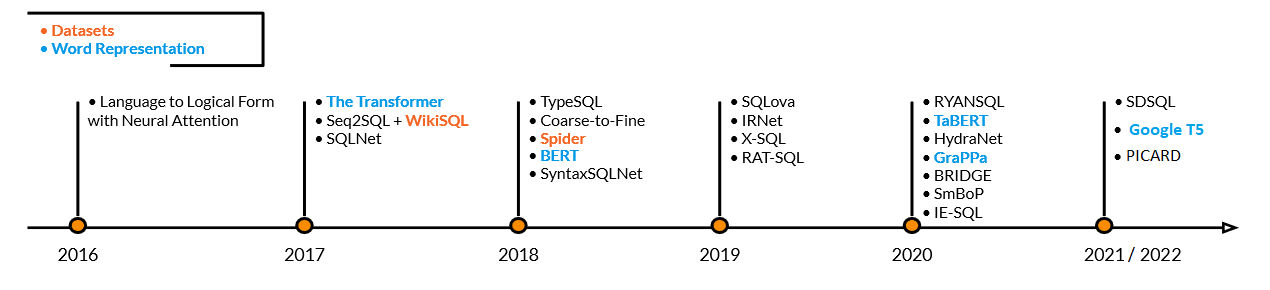
\includegraphics[width=1\textwidth]{pics/Timeline.png}
  \caption{\small Text-to-SQL over time}
  \label{fig:timeline}
\end{figure}

This section will discuss existing cross-domain state-of-the-art (SOTA), text-to-SQL models, beginning with a broad overview and moving on to individual modules.
% This will provide a clear picture of the progress made in text-to-SQL research. 

An efficient text-to-SQL solution requires state-of-the-art natural language processing techniques and Experiments have shown that pre-trained embeddings improve models because they construct better schema linking and a more accurate SQL structure.
As a result of the neural network's capacity to take only numerical inputs and not plain text, word embedding has been used to represent numerical words.
Aside from that, in the past few years, language models have evolved to become increasingly popular as a solution for increasing performance in natural language processing tasks.
Believing that words have numerical representations that differ from others, word embeddings aim to map each word to a multidimensional vector, incorporating valuable details about the word. In addition to the brute-force creation of one-hot embeddings, researchers have developed highly efficient methods for creating representations that convey a word's meaning and relationships with other words. In most, if not all, Text-to-SQL systems, word embedding techniques such as Word2Vec\cite{DBLP:journals/corr/Rong14}, and WordPiece embeddings\cite{DBLP:journals/corr/WuSCLNMKCGMKSJL16} are used.

Recently Language models have been shown to excel at NL tasks as a new type of pre-trained neural network. It is essential to note that language models are not a substitute for word embeddings since they are neural networks and need a way to transform words into vectors.
Relying on the specific problem they want to solve, researchers can adapt the pre-trained model's inputs and outputs and train it for an additional number of epochs on their dataset. Thus, we can achieve state-of-the-art performance without complex architectures \cite{DBLP:journals/corr/abs-1810-04805}. Recent neural network architectures, like the Transformer\cite{https://doi.org/10.48550/arxiv.1706.03762}, have been used to achieve such performance by these models, which excel at handling NL and sequences of NL that are characterized by connections between words. Several language models have been used to handle the text-to-SQL task, including BERT \cite{DBLP:journals/corr/abs-1810-04805}. BERT is a pre-trained language model that has been shown to achieve state-of-the-art performance in various NLP tasks. BERT is a Transformer-based model that utilizes a bidirectional encoder to understand the representation of a word based on the context in which it appears. BERT has been used in several text-to-SQL models, such as BRIDGE \cite{lin_bridging_2020} and RAT-SQL \cite{wang_rat_sql_2021}.

\clearpage
% \nofootrule
\begin{figure}
    \centering
    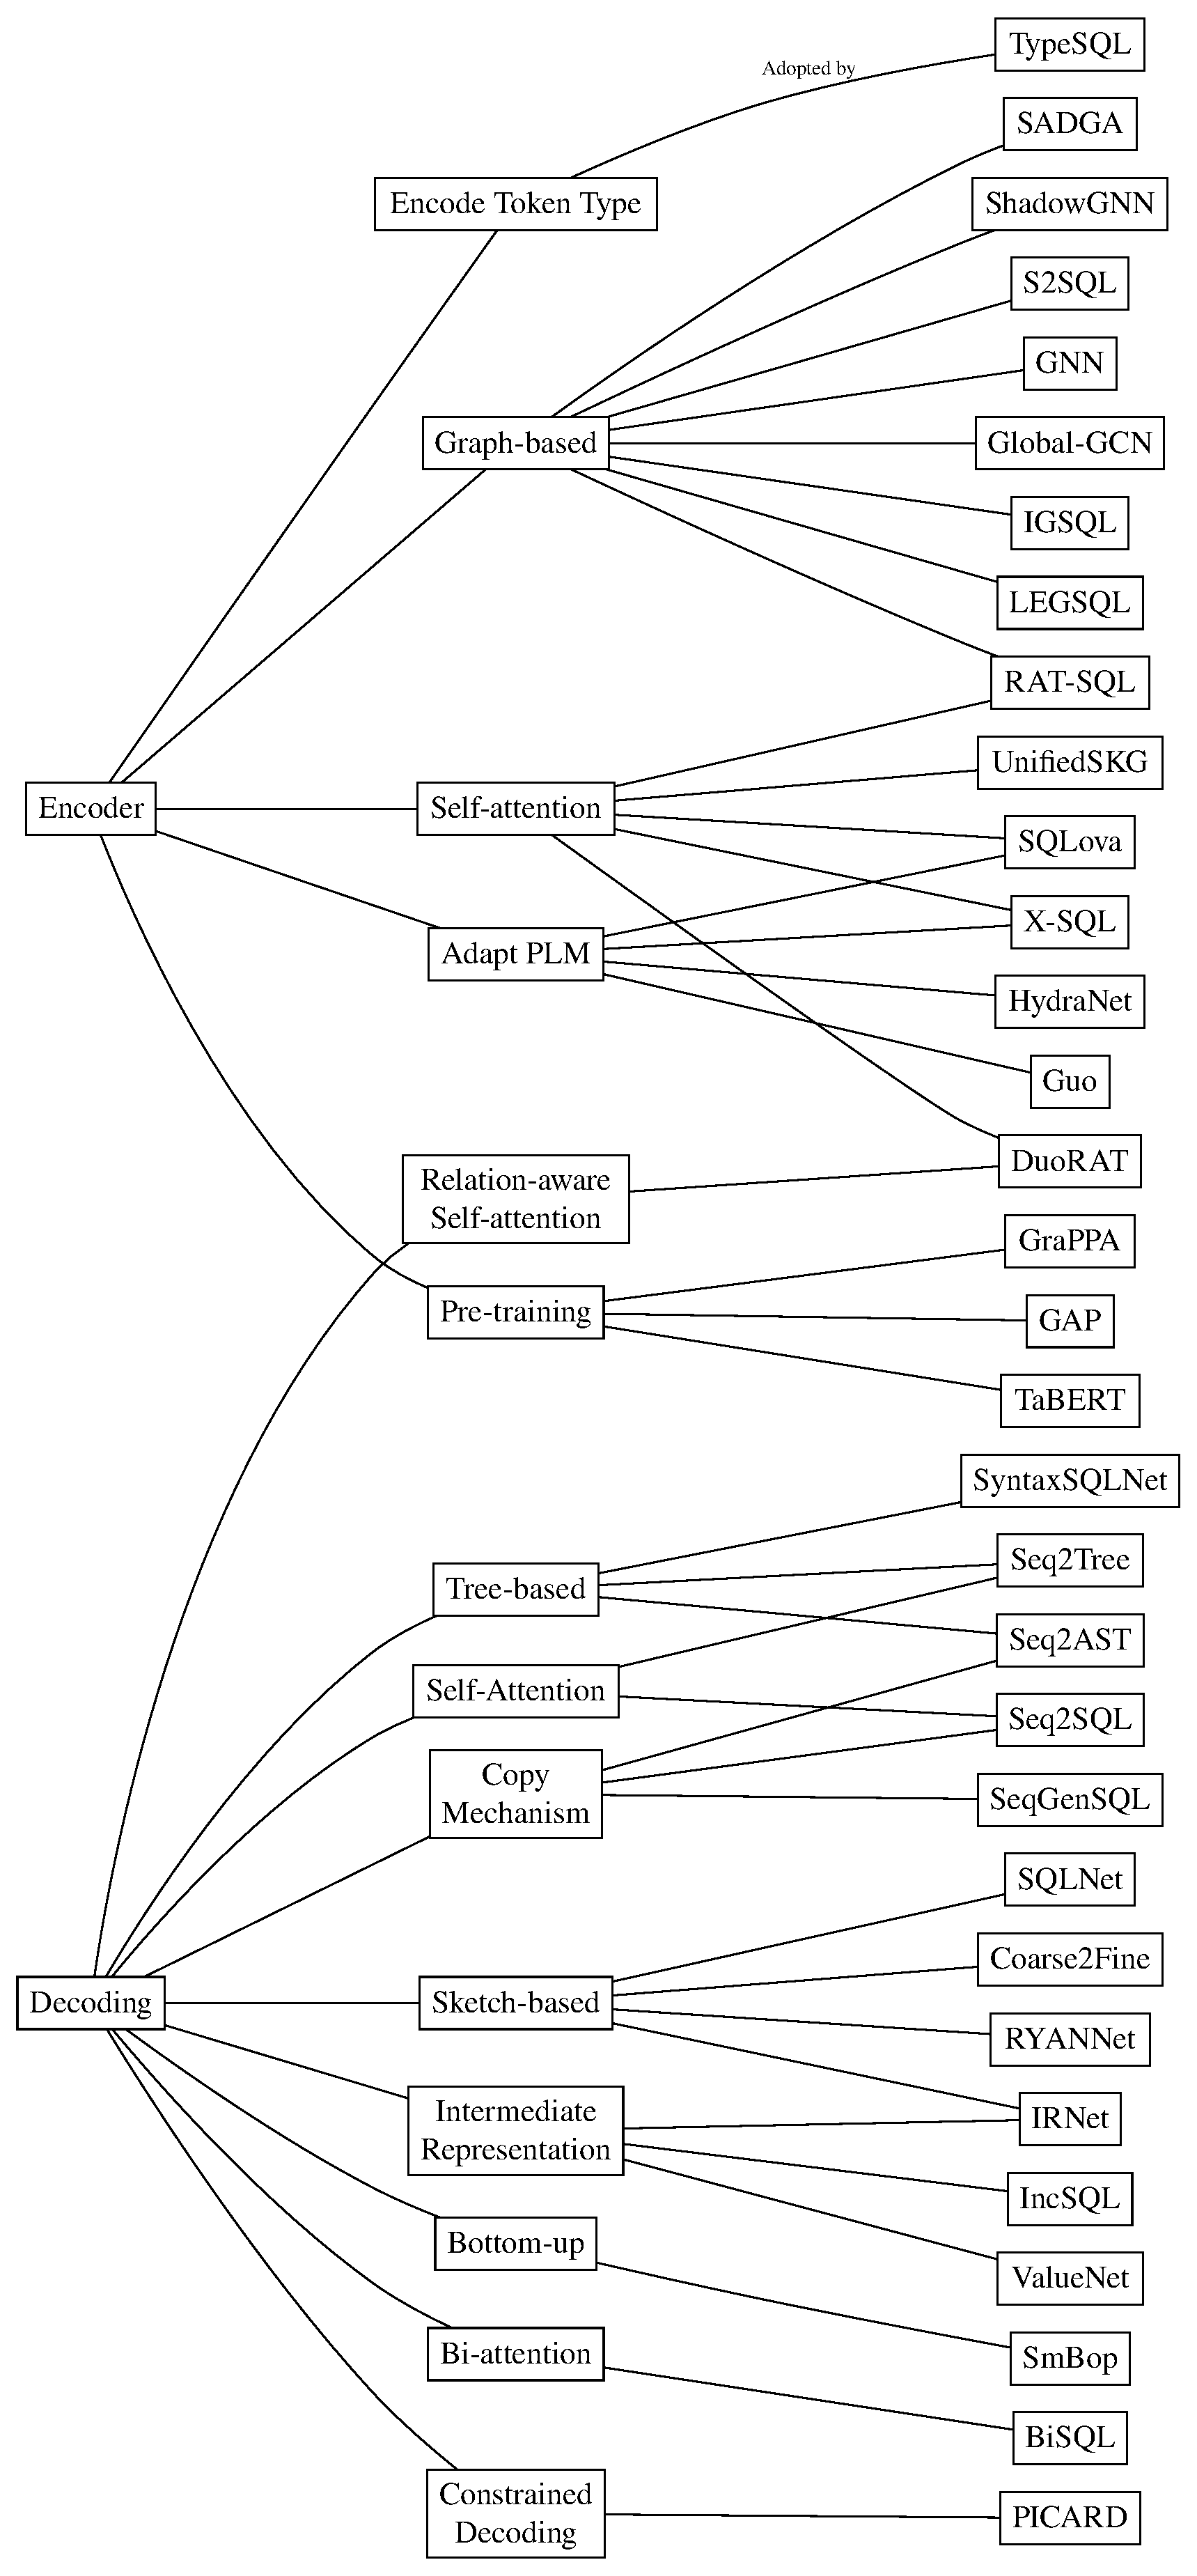
\includegraphics[height=0.98\textheight]{pics/mindmap/methods/map}
    \caption{\small{Text-to-SQL state-of-the-art Topology}}
    \label{fig:mindmap}
\end{figure}
\clearpage
\subsection{Encoding}
\label{sec:encoders}

% figure pics/transformer.jpg

\begin{figure}[H]
    \centering
    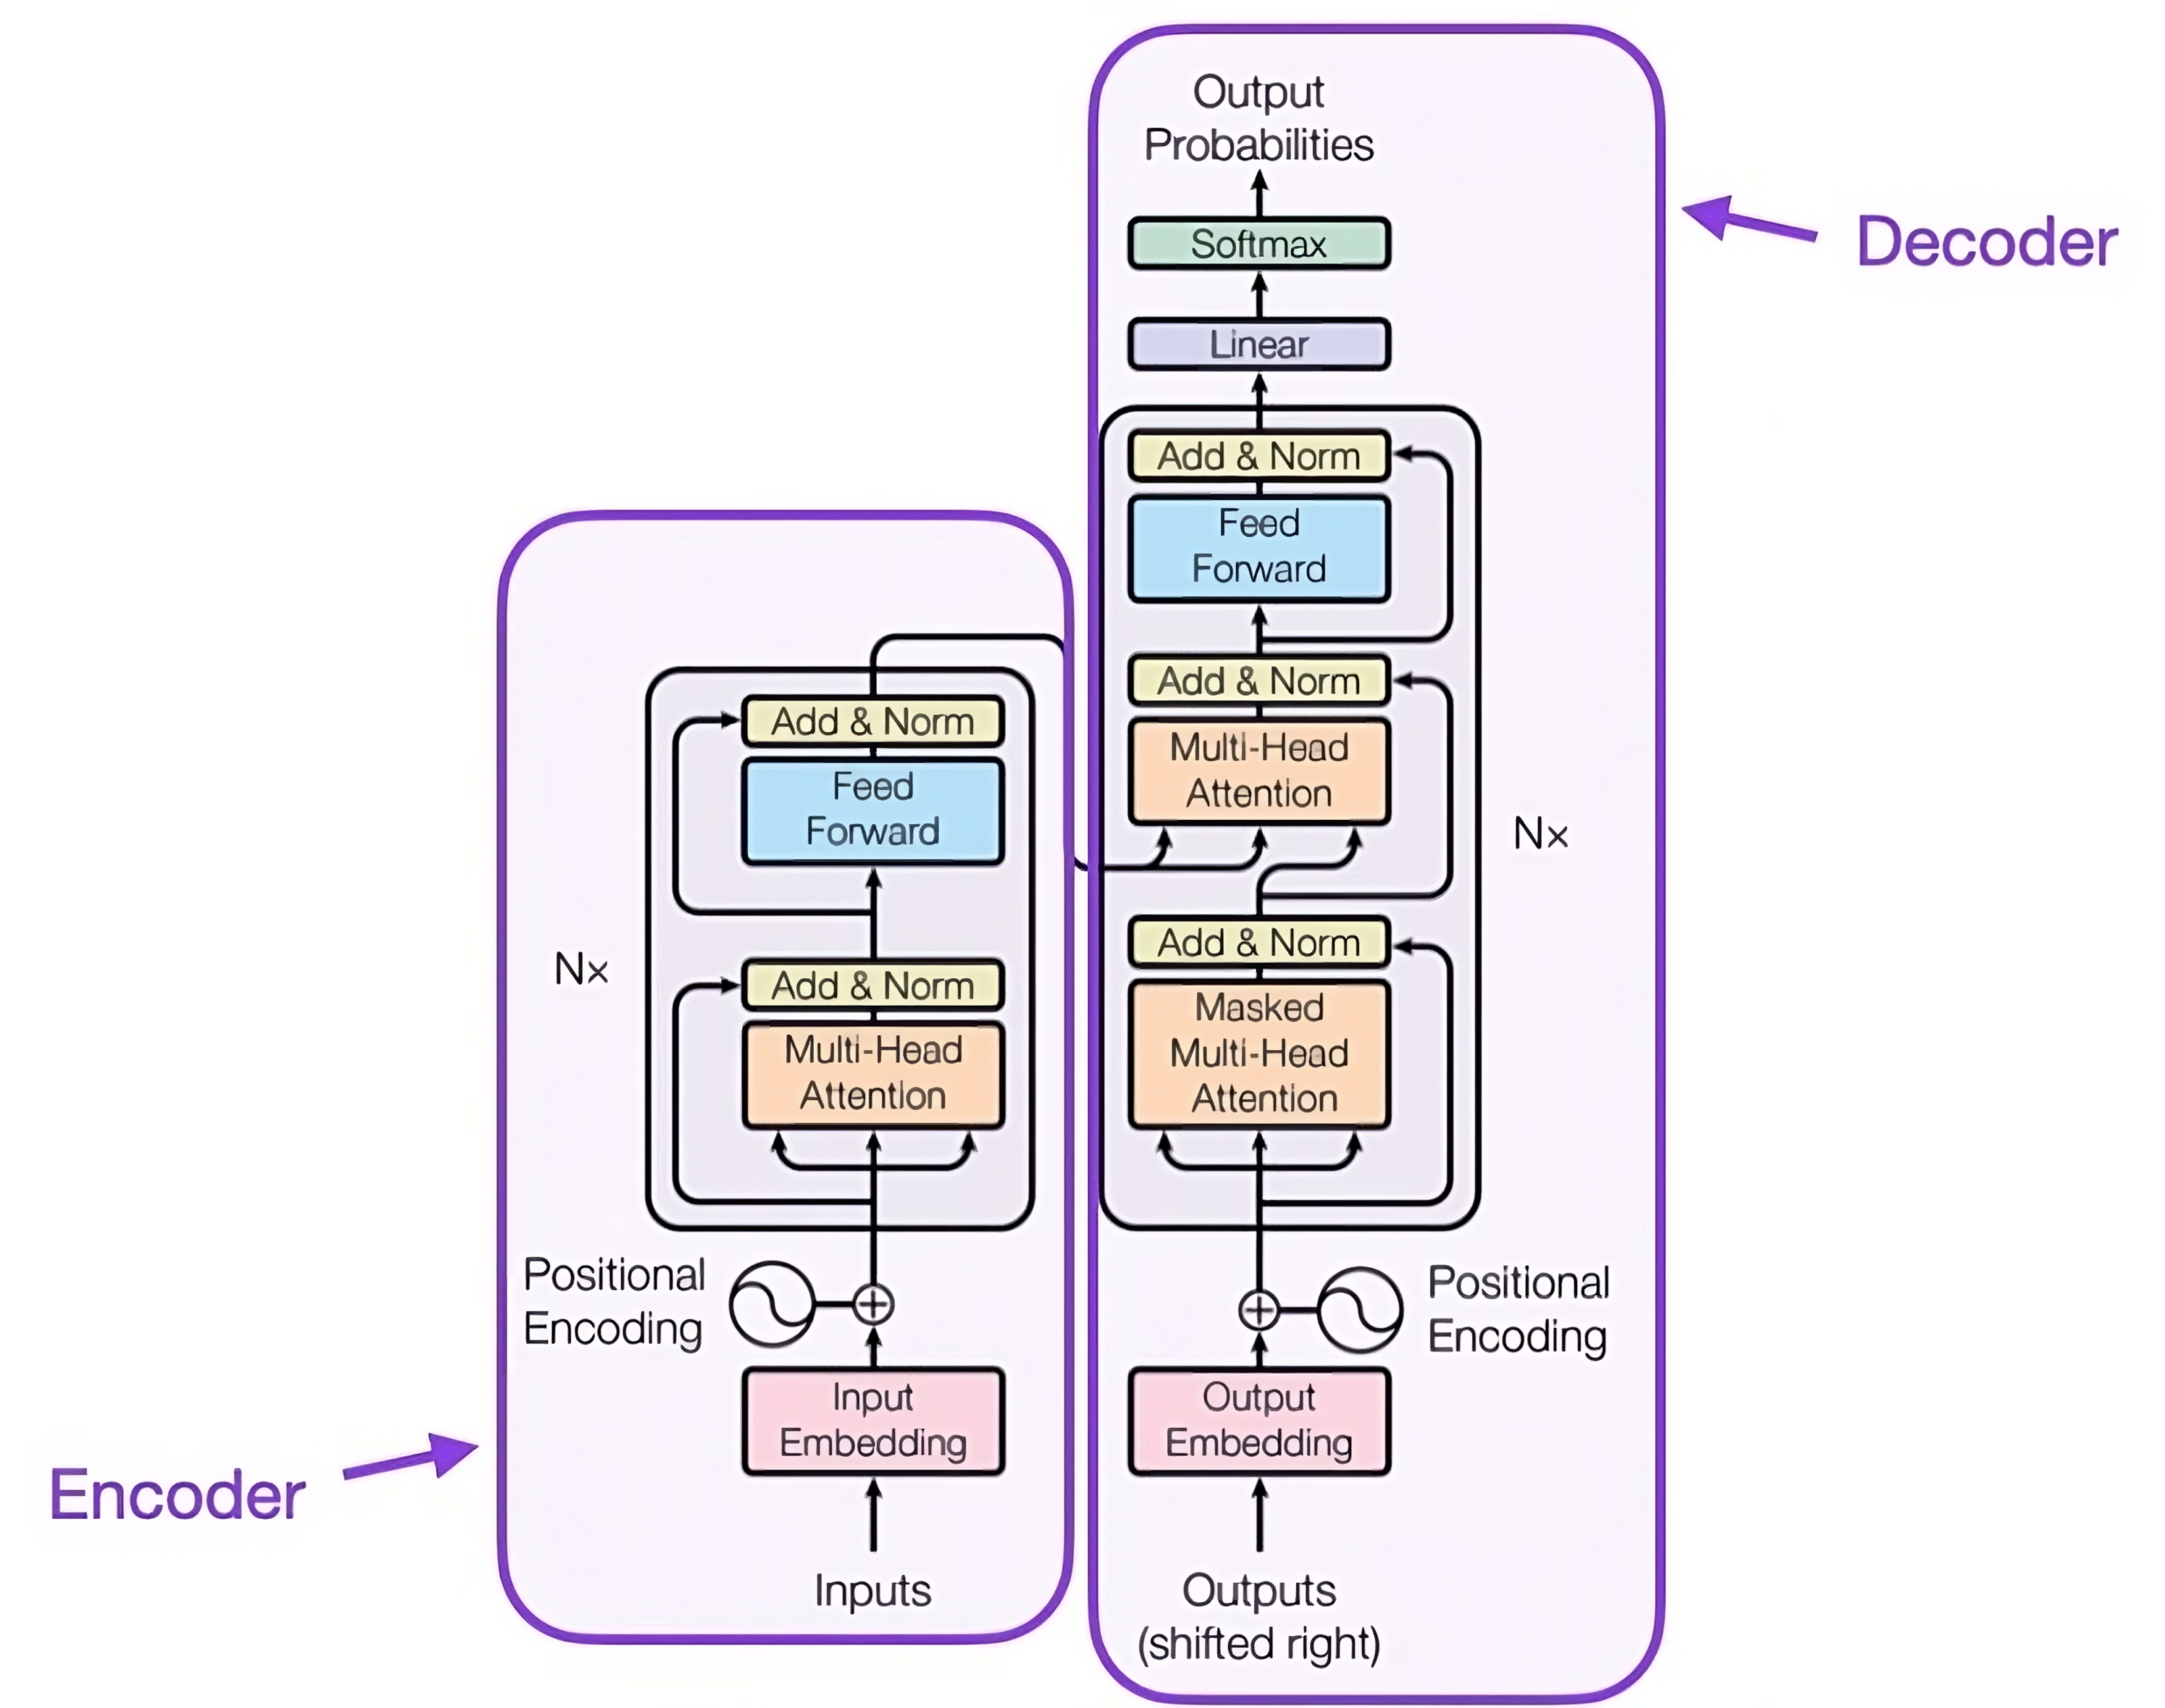
\includegraphics[width=0.8\linewidth]{pics/transformer-4x.jpg}
    \caption{Transformer architecture featured in “Attention is all you need” \cite{https://doi.org/10.48550/arxiv.1706.03762}}
    \label{fig:transformer}
\end{figure}

Encoders\cite{kumar2022deep} are a crucial component in natural language processing tasks and consist of a multi-layered assembly of recurrent elements, such as Long Short-Term Memory (LSTM) units, Gated Recurrent Units (GRUs), or other similar structures. These recurrent elements work in tandem to process an input sequence, with each unit being responsible for handling a single element within the sequence, capturing the pertinent information for that specific element, and subsequently propagating this information forward to the next recurrent unit in the stack.

The primary function of an encoder is to systematically transform textual data into a suitable numerical or vector representation that retains the inherent relationships and dependencies among words, phrases, and sentences\cite{cho-etal-2014-learning}. This is achieved through a combination of techniques, such as tokenization, embedding, and the use of attention mechanisms, which together facilitate the encoding process.

Tokenization serves to break down the input text into smaller, manageable units, such as words or subwords, while embeddings assign a dense vector representation to each token, thus allowing machines to efficiently process and compare these tokens. Attention mechanisms, on the other hand, enable encoders to weigh the importance of different input elements and selectively focus on the most relevant parts of the input sequence when generating the final encoded representation.

By effectively converting the textual data into a machine-understandable format, encoders play a pivotal role in empowering machines to recognize intricate patterns, relationships, and contextual cues within the text. Consequently, this ability to accurately discern the context of sentences and phrases forms the foundation for a wide array of natural language processing tasks, ranging from machine translation and sentiment analysis to text summarization and question-answering systems.

Several approaches have been explored to address the challenges of representing the meaning of questions, capturing the structure of database schemas, and establishing connections between database content and questions in the text-to-SQL domain\cite{deng2022recent}. These methods play a crucial role in facilitating the understanding of the complex relationships between natural language questions and their corresponding SQL queries.

One of the main challenges in text-to-SQL research is effectively representing the meaning of questions. Various encoding methods have been used to capture the semantics of natural language questions, ranging from traditional word embeddings like Word2Vec and GloVe to more advanced contextualized representations like BERT and its variants. These encoding techniques aim to produce meaningful vector representations of questions that models can use to understand and generate accurate SQL queries.

Another important aspect is representing database schemas, which serve as blueprints for organizing and structuring databases. Researchers have used various strategies to encapsulate database schema information, such as graph-based, tree-structured, and sequence-based encodings. These approaches enable text-to-SQL models to understand the hierarchical relationships and dependencies among various database elements. This allows for more accurate and efficient query generation.

Linking database content to questions is a vital task for text-to-SQL systems\cite{deng2022recent}. It involves the identification and mapping of relevant entities and attributes from the question to the database schema. To achieve this, various methods have been employed, including attention mechanisms, entity-linking techniques, and schema-agnostic encodings. These approaches help models identify relevant portions of the database schema and generate SQL queries that accurately reflect the intended meaning of the natural language questions.

Encoding methods and encoders play a crucial role in addressing the challenges of representing question semantics, encapsulating database schema structures, and linking database content to questions in the text-to-SQL domain. The exploration of diverse encoding techniques has led to significant advancements in the development of more accurate and efficient text-to-SQL models, furthering the field's understanding of the complex relationships between natural language questions and SQL queries\cite{deng2022recent}.

\begin{table}[H]
    \centering
    \newcolumntype{g}{>{\columncolor{Gray}}c}
    \begin{tabular}{|c|c|c|c|}
        \hline
        \rowcolor{Gray}
        \textbf{Methods}                & \textbf{Adopted by} & \textbf{Applied datasets} & \textbf{Addressed challenges}                                                                              \\
        \hline

        Encode token type               & TypeSQL             & WikiSQL                   & Representing question meaning                                                                              \\
        \hline
        \multirow{8}{*}{Graph-based}    & GNN                 & Spider                    & \multirow{8}{*}{\parbox{5cm}{Representing question and DB schemas in a structured way and Schema linking}} \\
                                        & Global-GCN          & Spider                    &                                                                                                            \\
                                        & IGSQL               & Sparc, CoSQL              &                                                                                                            \\
                                        & RAT-SQL             & Spider                    &                                                                                                            \\
                                        & LEGSQL              & Spider                    &                                                                                                            \\
                                        & SADGA               & Spider                    &                                                                                                            \\
                                        & ShawdowGNN          & Spider                    &                                                                                                            \\
                                        & S2SQL               & Spider                    &                                                                                                            \\
        \hline
        \multirow{5}{*}{Self-attention} & X-SQL               & WikiSQL                   & \multirow{5}{*}{\parbox{5cm}{Representing question and DB schemas in a structured way and Schema linking}} \\
                                        & SQLova              & WikiSQL                   &                                                                                                            \\
                                        & RAT-SQL             & Spider                    &                                                                                                            \\
                                        & DuoRAT              & Spider                    &                                                                                                            \\
                                        & UnifiedSKG          & WikiSQL, Spider           &                                                                                                            \\
        \hline
        \multirow{4}{*}{Adapt PLM}      & X-SQL               & WikiSQL                   & \multirow{4}{*}{\parbox{5cm}{Leveraging external data to represent question and DB schemas}}               \\
                                        & SQLova              & WikiSQL                   &                                                                                                            \\
                                        & Guo                 & WikiSQL                   &                                                                                                            \\
                                        & HydraNet            & WikiSQL                   &                                                                                                            \\
        \hline
        \multirow{3}{*}{Pre-training}   & TaBERT              & Spider                    & \multirow{3}{*}{\parbox{5cm}{Leveraging external data to represent question and DB schemas}}               \\
                                        & GraPPA              & Spider                    &                                                                                                            \\
                                        & GAP                 & Spider                    &                                                                                                            \\
        \hline
    \end{tabular}
    \caption{Methods used for encoding in text-to-SQL \cite{deng2022recent}}
    \label{tab:methods}
\end{table}

% \clearpage
\subsubsection{Encode Token Types}

\subsubsection{Graph-based Methods}

\subsubsection{Self-attention}
\label{sec:methods:encoders:SelfAttention}

Self-attention is a fundamental component in natural language processing (NLP) models, particularly those based on the Transformer architecture. It serves as the primary building block of the transformer structure, as mentioned in the works of X-SQL\cite{he2019xsql}, SQLova\cite{DBLP:journals/corr/abs-1902-01069}, and UnifiedSKG\cite{xie2022unifiedskg}. These models employ the original self-attention mechanism by default.

The self-attention mechanism allows the model to weigh and aggregate different words or tokens in a sequence based on their relative importance\cite{https://doi.org/10.48550/arxiv.1706.03762}. In essence, it helps the model to focus on the most relevant parts of a given input while processing it. This is accomplished by computing attention scores between each pair of tokens in the input, which are then used to produce a weighted sum of the input tokens. The mechanism is particularly effective in handling long-range dependencies within the text.

However, the original self-attention mechanism can be modified to cater to specific tasks or address particular challenges. One such modification is relation-aware self-attention, employed by RAT-SQL\cite{wang_rat_sql_2021} and DuoRAT\cite{scholak-etal-2021-duorat}. This variation of self-attention is designed to take advantage of the relationships between tables and columns when working with structured data.

Relation-aware self-attention extends the original self-attention by incorporating information about the structure and relations in the input data. This additional information is used to adjust the attention scores, allowing the model to focus on the most relevant relationships between different elements in the input. As a result, models equipped with relation-aware self-attention can better handle tasks involving structured data, such as SQL query generation or table-based reasoning.

% \begin{table}[t]
%     \centering
%     \scalebox{0.8}{
%         \begin{tabular}{lcc}
%             \toprule
%             \textbf{Model}                                 & \textbf{EMA Dev.} \\
%             \midrule
%             X-SQL\cite{he2019xsql}                         & 89.5              \\
%             SQLova\cite{DBLP:journals/corr/abs-1902-01069} & 87.2              \\
%             RATSQL \cite{wang_rat_sql_2021}                & 69.7              \\
%             UnifiedSKG\cite{xie2022unifiedskg}             & 72.3              \\
%             DuoRAT\cite{scholak-etal-2021-duorat}          & 75.1              \\
%             \bottomrule
%         \end{tabular}
%     }
%     \caption{The exact match accuracy on the Spider dev set.}
%     \label{table:methods:encoders:SelfAttention}
% \end{table}
\subsubsection{Adapt PLM} %Pre-trained Language Models
\label{sec:adaptplm}

\begin{figure*}[htbp]
    \centering
    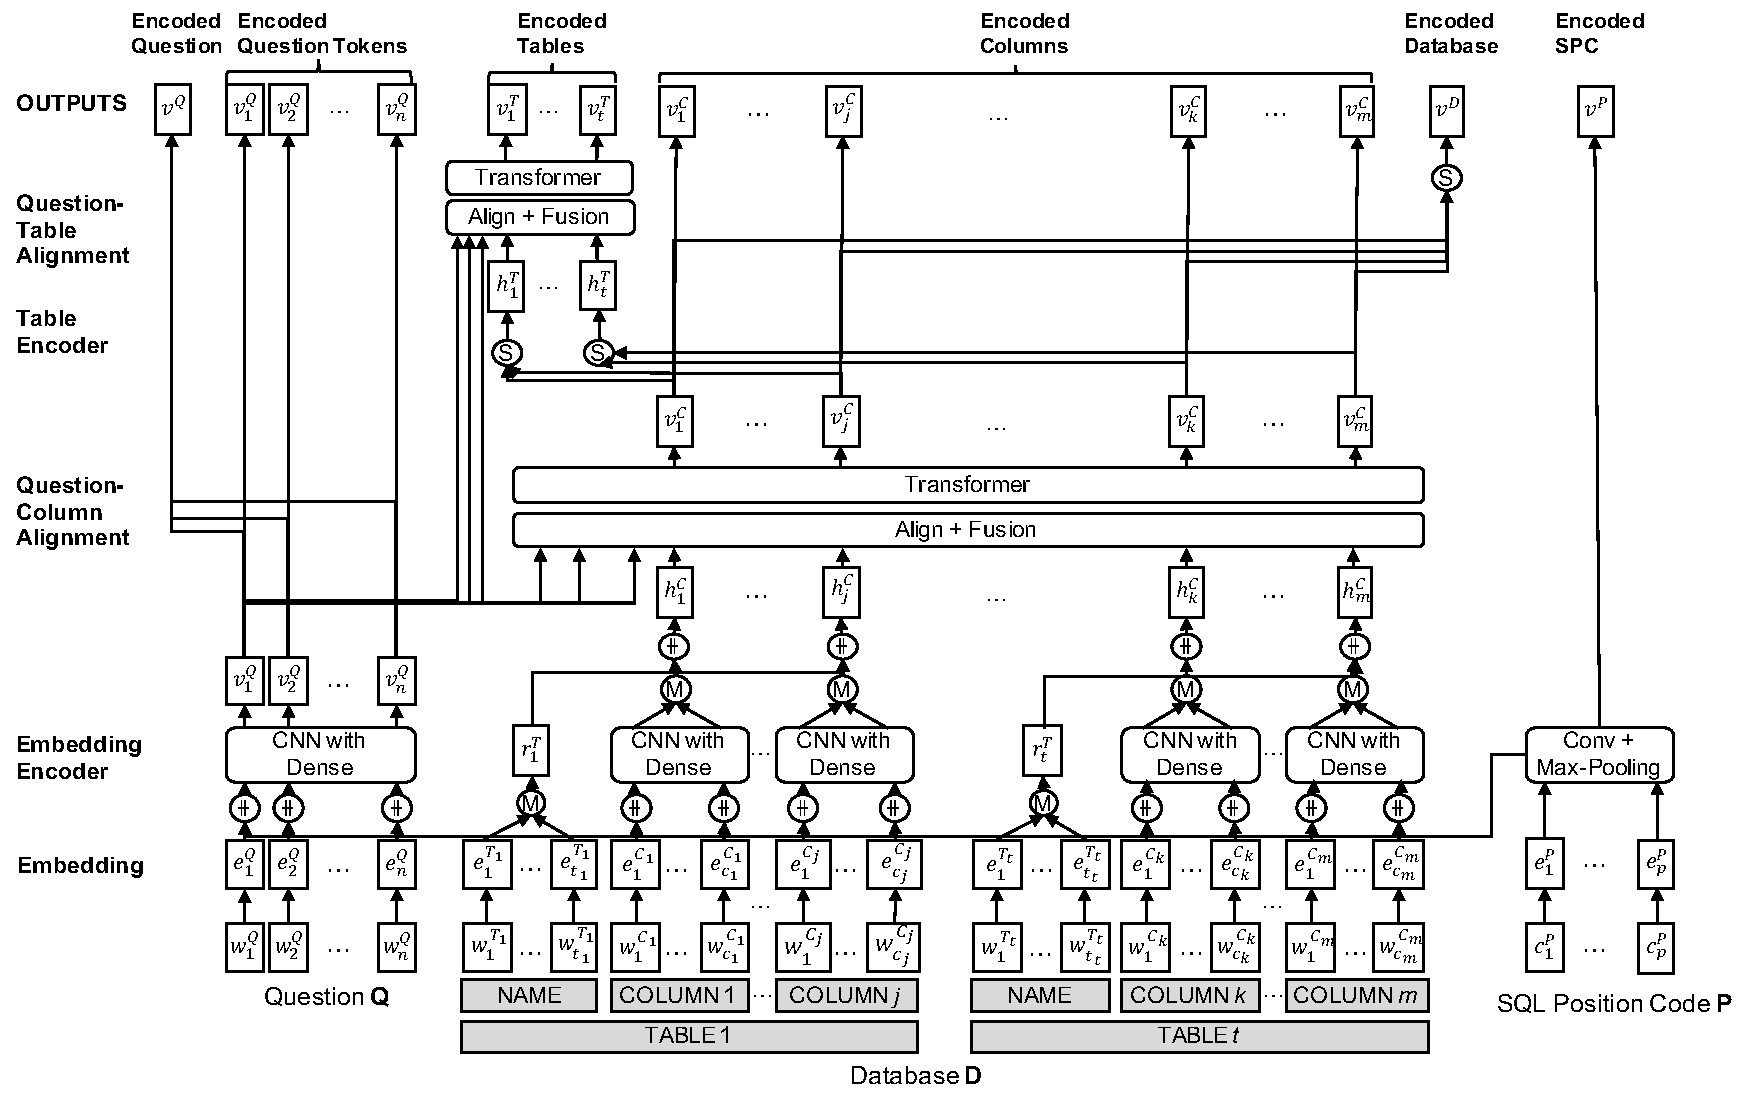
\includegraphics[width=\textwidth]{pics/enc/fig_encode}
    \caption{Network architecture of the proposed input encoder. \raisebox{-0.5ex}{
\includegraphics[height=3.3mm]{pics/enc/mark_1}} represents vector concatenation, \raisebox{-0.5ex}{
\includegraphics[height=3.3mm]{pics/enc/mark_2}} represents max-pooling and \raisebox{-0.5ex}{
\includegraphics[height=3.3mm]{pics/enc/mark_3}} represents self-attention.\cite{choi_ryansql_2020}}
    \label{fig:ryan}
\end{figure*}

Adapt \ac{PLM} methods aim to utilize the knowledge encapsulated in pre-trained language models, such as BERT\cite{DBLP:journals/corr/abs-1810-04805}, to improve their performance on text-to-SQL tasks. These methods modify or extend the original PLMs to better align with the specific requirements of the task.

One common approach is to encode both the natural language questions and the database schemas using PLMs. For instance, SQLova\cite{DBLP:journals/corr/abs-1902-01069} and RYANSQL\cite{10.1162/coli_a_00403} concatenate the question words and schema words as input to the BERT encoder. This approach allows the model to learn representations that capture the relationships between questions and the underlying schema. In figure \ref{fig:ryan}, the authors of RYANSQL\cite{10.1162/coli_a_00403} propose a novel encoder that combines the BERT encoder with a self-attention mechanism to capture the interactions between the question and schema words. As you can see it passes the question words and database tables schemas through embedding layers, then concatenates them and passes them through the BERT encoder. The output of the BERT encoder is then passed through a self-attention layer to capture the interactions between the question and schema words. The self-attention layer is then concatenated with the BERT encoder output and passed through a feed-forward network to produce the final representation of the question and schema.

Some methods go a step further by adjusting the embeddings produced by the PLMs. X-SQL\cite{he2019xsql} proposes the replacement of the segment embeddings from the pre-trained encoder with column-type embeddings for the WikiSQL dataset. Guo and Gao \cite{guo2020content} introduce an approach that encodes additional feature vectors for matching between question tokens and table cells, as well as column names. These feature vectors are then concatenated with the BERT embeddings of questions and DB schemas.

HydraNet\cite{lyu_hybrid_2020} uses BERT to encode the question and individual columns, an approach that is more aligned with the tasks BERT is pre-trained on. After obtaining BERT representations for all columns, the model selects the top-ranked columns for SQL prediction


\begin{table}[t]
    \centering
    \scalebox{0.8}{
        \begin{tabular}{lcc}
            \toprule
            \textbf{Model}                                  & \textbf{Execution Accuracy} \\
            Seq2SQL\cite{zhong_seq2sql_2017}                & 60.8                        \\
            TypeSQL\cite{DBLP:journals/corr/abs-1804-09769} & 74.5                        \\
            \midrule
            SQLova\cite{DBLP:journals/corr/abs-1902-01069}  & 90.2                        \\
            Guo\cite{guo2020content}                        & 91.1                        \\
            HydraNet\cite{lyu_hybrid_2020}                  & 92.4                        \\
            \bottomrule
        \end{tabular}
    }
    \caption{The execution accuracy on the WikiSQL dev set.}
    \label{table:methods:encoders:adaptplm}
\end{table}

Examining the WikiSQL benchmark results in Table \ref{table:methods:encoders:adaptplm}, we can observe a significant overall performance improvement when employing pre-trained language models (PLMs) compared to previous methods. This enhancement can be attributed to the ability of PLMs, such as BERT, to capture complex linguistic patterns and relationships within the input data. By leveraging the knowledge encapsulated in these models and adapting them to the text-to-SQL task, researchers have been able to achieve better alignment with the specific requirements of the problem domain. As a result, PLM-based approaches have demonstrated superior performance in generating accurate SQL queries from natural language questions, surpassing traditional methods and showcasing the potential of PLMs in addressing complex language understanding tasks.

\subsubsection{Pre-training}



\clearpage
\subsection{Decoding}

Decoders \cite{cho-etal-2014-learning} form an integral part of sequence-to-sequence models in natural language processing tasks, and they are constructed as a multi-layered architecture of recurrent elements, such as Long Short-Term Memory (LSTM) units, Gated Recurrent Units (GRUs), or other analogous structures. The primary responsibility of a decoder is to generate an output sequence by predicting an output, denoted as y, for each time step. This output sequence can be a series of words, phrases, or even entire sentences, depending on the specific problem being addressed.

At each time step, the current recurrent unit within the decoder receives a hidden state from the preceding recurrent unit. This hidden state encapsulates the information gathered up to that point and serves as a vital input for the current recurrent unit to make an informed prediction. Moreover, decoders can also incorporate attention mechanisms to help focus on the most relevant parts of the input sequence when generating the output. This is particularly useful in tasks that require the decoder to selectively attend to different input elements during the decoding process.

Decoders are commonly employed in a wide range of natural language processing applications \cite{kumar2022deep}, including but not limited to, machine translation, text summarization, question-answering systems, and dialogue generation. In question-answering tasks, for instance, the output sequence generated by the decoder is often a collection of words.

Numerous approaches have been suggested to enhance the decoding process for more precise and efficient SQL generation, ultimately bridging the divide between natural language and SQL query formulation. As illustrated in the table below, we have classified these techniques into five primary categories, along with additional methodologies\cite{deng2022recent}.

\begin{table}[H]
    \centering
    \begin{tabular}{cccc}
        \hline
        \rowcolor{Gray}
        \textbf{Methods}                                           & \textbf{Adopted by} & \textbf{Applied datasets} & \textbf{Addressed challenges}                                                            \\
        \hline
        \multirow{3}{*}{Tree-based}                                & Seq2Tree            & -                         & \multirow{3}{*}{Hierarchical decoding}                                                   \\
                                                                   & Seq2AST             & -                         &                                                                                          \\
                                                                   & SyntaxSQLNet        & Spider                    &                                                                                          \\
        \hline
        \multirow{4}{*}{Sketch-based}                              & SQLNet              & WikiSQL                   & \multirow{4}{*}{Hierarchical decoding}                                                   \\
                                                                   & Coarse2Fine         & WikiSQL                   &                                                                                          \\
                                                                   & IRNet               & Spider                    &                                                                                          \\
                                                                   & RYANSQL             & Spider                    &                                                                                          \\
        \hline
        Bottom-up                                                  & SmBop               & Spider                    & Hierarchical decoding                                                                    \\
        \hline
        \multirow{2}{*}{Self-Attention}                            & Seq2Tree            & -                         & \multirow{2}{*}{ Synthesizing information}                                               \\
                                                                   & Seq2SQL             & WikiSQL                   &                                                                                          \\
        \hline
        Bi-attention                                               & BiSQL               & Spider                    & Synthesizing information                                                                 \\
        \hline
        \parbox{3cm}{Relation-aware Self-attention}                & DuoRAT              & Spider                    & Synthesizing information                                                                 \\
        \hline
        \multirow{3}{*}{Copy Mechanism}                            & Seq2AST             & -                         & \multirow{3}{*}{ Synthesizing information}                                               \\
                                                                   & Seq2SQL             & WikiSQL                   &                                                                                          \\
                                                                   & SeqGenSQL           & WikiSQL                   &                                                                                          \\
        \hline
        \multirow{3}{*}{\parbox{3cm}{Intermediate Representation}} & IncSQL              & WikiSQL                   & \multirow{3}{*}{{\parbox{5cm}{Bridging the gap between natural language and SQL query}}} \\
                                                                   & IRNet               & WikiSQL                   &                                                                                          \\
                                                                   & ValueNet            & Spider                    &                                                                                          \\
        \hline
        Constrained decoding                                       & PICARD              & Spider                    & Fine-grained decoding                                                                    \\
        % \hline
        % Execution-guided                                           & SQLova              & WikiSQL                   & Fine-grained decoding                                                                    \\
        % \hline
        % Separate submodule                                         & SQLNet              & WikiSQL                   & Easier decoding                                                                          \\
        % \hline
        % BPE                                                        & BPESQL              & Advising, ATIS
        %    & Easier decoding
        % \\
        \hline
    \end{tabular}
    \caption{Methods used for decoding in text-to-SQL \cite{deng2022recent}}
    \label{tab:decoders}
\end{table}

% \clearpage
\subsubsection{Tree-based}

\subsubsection{Sketch-based}

Sketch-based decoders have gained attention in text-to-SQL research as an approach that simplifies the generation of SQL queries by leveraging predefined query structures, or "sketches." These sketches follow SQL grammar and allow the model to focus on filling in the slots rather than predicting the output grammar and content simultaneously.

SQLNet by Xu et al.  \cite{xu_sqlnet_2017} is an example of a sketch-based model that aligns with SQL grammar. The sketch captures dependencies between predictions, which means that the prediction for each slot is conditioned only on the slots it depends on. This approach effectively avoids issues arising from equivalent serializations of the same SQL query.

Dong and Lapata  \cite{dong-lapata-2018-coarse} further refine the sketch-based approach by decomposing the decoding process into two stages. The first decoder predicts a rough sketch, while the second decoder fills in the low-level details based on the input question and the sketch. This coarse-to-fine decoding has been adopted in other works, such as IRNet by Guo et al.  \cite{DBLP:journals/corr/abs-1905-08205}.

To handle complex SQL queries with nested structures, RYANSQL by Choi et al.  \cite{10.1162/coli_a_00403} introduces a recursive method for generating SELECT statements. This model employs sketch-based slot filling for each of the SELECT statements, enabling the generation of more intricate queries.

In summary, sketch-based decoders simplify the text-to-SQL generation process by providing predefined query structures that follow SQL grammar. This approach enables models to focus on filling in content slots, captures dependencies between predictions, and allows for the handling of complex queries with nested structures. By decomposing the decoding process into multiple stages, sketch-based decoders can efficiently translate natural language questions into accurate SQL queries.
\subsubsection{Bottom-up}

\subsubsection{Attention Mechanism}

Attention mechanism decoders play a critical role in integrating encoder-side information during the decoding process. By computing attention scores and multiplying them with hidden vectors from the encoder, a context vector is generated, which is then used to produce an output token.

Various attention structures have been employed to enhance the decoder's performance and effectively propagate the information encoded from questions and database schemas. One such example is SQLNet (Xu et al., 2017) \cite{xu_sqlnet_2017}, which introduces the concept of column attention. This technique involves using hidden states from columns and multiplying them by embeddings for the question to calculate attention scores for a given column. The attention scores are then used to help the model focus on relevant columns when generating the SQL query.

Another approach, proposed by Guo and Gao (2018) \cite{guo2020content}, incorporates bi-attention over a question and column names for SQL component selection. This method enables the model to simultaneously attend to both the question and column names, which can improve the model's ability to identify and select relevant SQL components.

Wang et al. (2019) \cite{wang-etal-2019-learning} adopt a structured attention mechanism \cite{kim2017structured} that computes marginal probabilities to fill in the slots of their generated abstract SQL queries. This approach allows the model to better capture the structure of SQL queries and enhances the overall generation process.

DuoRAT \cite{scholak-etal-2021-duorat} implements a relation-aware self-attention mechanism in both its encoder and decoder components. This attention mechanism accounts for relationships between different elements within the input data, thus improving the model's ability to comprehend and generate accurate SQL queries.

Other works, such as those by Scholak et al. PICARD (2021b) \cite{Scholak2021:PICARD} and UnifiedSKG by Xie et al. (2022) \cite{xie2022unifiedskg}, use sequence-to-sequence transformer-based models or decoder-only transformer-based models that incorporate the self-attention mechanism by default. The self-attention mechanism allows the model to weigh the significance of each input token concerning other tokens in the sequence, which can enhance the quality and coherence of the generated output.

In summary, attention mechanism decoders have been an essential aspect of Text-to-SQL research, with various structures designed to improve the propagation of information and the generation of accurate SQL queries. By continuously refining and adapting these attention mechanisms, researchers aim to further enhance the performance of Text-to-SQL models.
\subsubsection{Copy Mechanism}

\subsubsection{Intermediate Representations}

Intermediate representations (IRs) are employed in Text-to-SQL research to bridge the gap between natural language and SQL queries. By using IRs, researchers can simplify and abstract SQL queries, making it easier for models to learn and generate an accurate output.

IncSQL by Shi et al. (2018)\cite{shi2018incsql} is one such approach that defines actions for different SQL components, allowing the decoder to decode these actions instead of raw SQL queries. This method reduces the complexity of the decoding process and can improve the overall performance of the model.

IRNet by Guo et al. (2019) \cite{DBLP:journals/corr/abs-1905-08205} introduces SemQL, an intermediate representation for SQL queries designed to cover most of the challenging Spider benchmark. SemQL simplifies SQL queries by removing the JOIN ON, FROM, and GROUP BY clauses and merging the HAVING and WHERE clauses. ValueNet by Brunner and Stockinger (2021) \cite{brunner2021valuenet} builds upon SemQL by introducing SemQL 2.0, which extends the original representation to include value representation. Additionally, NatSQL by Gan et al. (2021c) \cite{gan-etal-2021-natural-sql} modifies SemQL by removing set operators, such as INTERSECT, which combine the results of two or more SELECT statements.

Suhr et al. (2020) \cite{semql} implement SemQL as a mapping from SQL to a representation with an under-specified FROM clause, which they call SQLUF. Rubin and Berant (2021) employ a relational algebra augmented with SQL operators as intermediate representations, offering another approach to simplifying SQL queries.

However, one of the main challenges with intermediate representations is that they are typically designed for specific datasets and cannot be easily adapted to others. To address this issue, Herzig et al. (2021) \cite{herzig2021unlocking} propose a more generalized intermediate representation by omitting tokens in the SQL query that do not align with any phrase in the natural language utterance.

The success of intermediate representations in Text-to-SQL tasks has inspired researchers to explore their use in other executable language domains, such as SPARQL for database systems. Works by Saparina and Osokin (2021) \cite{saparina-osokin-2021-sparqling} investigate the potential of intermediate representations for SPARQL queries.

In conclusion, intermediate representations play an essential role in Text-to-SQL research by simplifying and abstracting SQL queries, making it easier for models to learn and generate an accurate output. The exploration of various intermediate representation techniques continues to improve the performance of Text-to-SQL models and inspire advancements in other related domains.
\subsubsection{Constrained decoding}

Constrained decoding methods are employed in natural language processing tasks, such as text-to-SQL, to improve the quality of generated outputs by imposing certain constraints or utilizing auxiliary models during the decoding process. These methods aim to prevent the generation of invalid tokens, exclude non-executable partial SQL queries, or facilitate the generation of complete SQL queries.

PICARD by Scholak et al., \cite{Scholak2021:PICARD} is an example of a method that sets constraints on the decoder to avoid generating invalid tokens. Other methods, such as those proposed by Wang et al. \cite{wang2018robust} and Hwang et al. \cite{DBLP:journals/corr/abs-1902-01069}, adopt an execution-guided decoding mechanism that eliminates non-executable partial SQL queries from the output candidates.

Some approaches, like Global-GNN, Bogin et al. \cite{bogin-etal-2019-global}, use separately trained discriminative models to rerank the top-K SQL queries in the decoder's output beam. This technique allows the model to reason about complete SQL queries rather than considering each word and database schema in isolation.

Chen et al. \cite{chen-etal-2020-tale} employ a gating mechanism to select between the output sequence encoded for the question and the output sequence from the previous decoding steps at each step for SQL generation. This approach helps in generating more accurate and coherent SQL queries.

Müller and Vlachos \cite{müller2019bytepair} draw inspiration from machine translation and apply \ac{BPE} (Sennrich et al.\cite{sennrich-etal-2016-neural}) to compress SQL queries into shorter sequences, guided by AST. This technique reduces the difficulties in SQL generation, leading to improved performance in text-to-SQL tasks.


% Schema linking is a component of text-to-SQL models that helps map natural language phrases to elements of a database schema.
% Skeleton parsing is a component of text-to-SQL models that helps generate the structure of an SQL query based on a natural language question. It focuses on generating the pure skeleton of an SQL query (i.e., SQL keywords).
% \clearpage
\section{Data Augmentation}
\label{sec:augmentation}


\subsection{Evaluation method}

Text-to-SQL tasks can be evaluated by two methods: accurate matching rate and execution accuracy rate. Predicted SQL statements are compared with standard statements to determine how accurate the match is.
By splitting the predicted SQL statement and definitive statement into multiple clauses according to keywords, we can solve the problem of matching errors caused by order of the where clause. The matching is successful as long as the elements in both sets are the same.

% pics/acc1.png
\begin{figure}[htb]
    \centering
    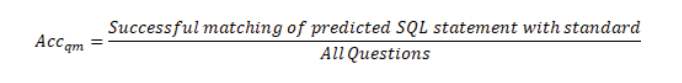
\includegraphics[width=0.6\textwidth]{pics/acc1.png}
    % \caption{Accurate matching rate}
    \label{fig:acc1}
\end{figure}

When using the correct predicted SQL statements, the correct execution rate refers to the proportion of questions that can receive the correct answers from the database.

% pics/acc2.png
\begin{figure}[htb]
    \centering
    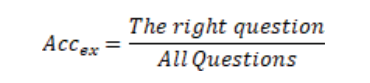
\includegraphics[width=0.4\textwidth]{pics/acc2.png}
    % \caption{Accuracy rate of the predicted SQL statements}
    \label{fig:acc2}
\end{figure}

By predicting the key F1 values for SQL statements, the model can also be evaluated.

% pics/f1.png
\begin{figure}[htb]
    \centering
    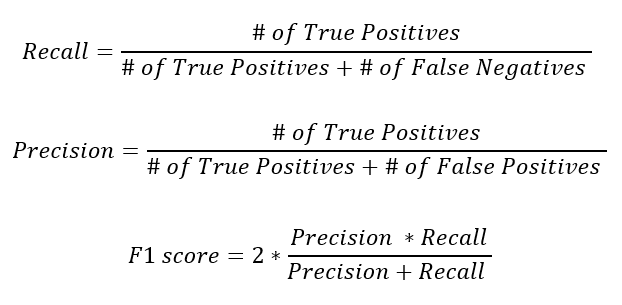
\includegraphics[width=0.6\textwidth]{pics/f1.png}
    % \caption{F1 score for SQL statements}
    \label{fig:f1}
\end{figure}
\section{Experiments}

Since the SEOSS Dataset\cite{RATH2019104005} has only been evaluated and trained with SQLNet and RatSQL, in this section, we aim to further explore its potential by conducting experiments using state-of-the-art methods currently proposed for the SPIDER challenge. To assess the effectiveness of these approaches, we compare the outcomes with those of SQLNet and RatSQL, as reported in the SEOSS-Queries research paper\cite{TOMOVA2022108211}. The findings from these experiments are detailed in the subsequent section, showcasing the capabilities of contemporary solutions in tackling the SPIDER task.

Additionally, taking advantage of the publicly available ChatGPT APIs, we decided to experiment with the ChatGPT model. Employing both the SPIDER and SEOSS datasets, we compared the results with those obtained from earlier experiments. The insights derived from these experiments are presented in the following section, further illustrating the potential of modern solutions in addressing the SPIDER task.

\subsection{Limitations}

Our experiment faced several limitations, primarily due to the extensive computational resources required when leveraging the T5 model. For our experiment, we used a single Nvidia RTX 3070 16GB GPU with 20GB Memory, which constrained us to smaller models with tighter restrictions. Despite these limitations, we managed to achieve admirable results. Utilizing a larger T5 model could have led to even higher scores. As a result, investing in a more powerful GPU for our experiment should be considered to capitalize on our model's potential fully.
In addition, during the ChatGPT experiment, cost constraints limited our ability to experiment with GPT-4.0, as its usage cost is approximately 30 times higher than that of GPT-3.5-turbo. We had to experiment with different methods to find the best prompt for ChatGPT to force him to act as a text-to-SQL agent, but this led to wasting money.

\begin{table}[h]
    \centering
    \begin{tabular}{|l|l|}
        \hline \textbf{Model} & \textbf{Usage}      \\
        \hline GPT-4          & \$0.06 / 1K tokens  \\
        \hline GPT-3.5-turbo  & \$0.002 / 1K tokens \\
        \hline
    \end{tabular}
    \caption{Cost comparison between GPT-4 and GPT-3.5-turbo}
    \label{tab:cost_comparison}
\end{table}

\subsection{SEOSS evaluation with T5 PICARD}

\begin{figure}[H]
    \begin{AIbox}{Additional Materials}
        \parbox{1\textwidth}{
            The code and evaluated experiment results are detailed in the provided GitHub repository and the CD attached to this thesis.
        }
    \end{AIbox}
\end{figure}

After studying the SEOSS dataset, we decided to experiment with the PICARD model\ref{picard} to evaluate its performance against that of SQLNet and RatSQL. We decided to use the T5-Base and T5-Large models for our experiment, as they are smaller than the T5-3B and T5-11B models used by most state-of-the-art studies. To ensure a fair comparison between the models, we used two beam sizes of 2 and 4 and the same evaluation metrics as SEOSS-SQLNet and SEOSS-RatSQL, which is "exact matching accuracy". We wanted to see if the PICARD model could achieve similar results to those of SQLNet and RatSQL, so we conducted our experiment with our findings. The results of our experiment are discussed in the following section and can be used to compare the performance of the PICARD model to the models used in the SEOSS study.
\footnote[1]{Link to the Github Page: \url{https://github.com/yazdipour/text-to-sql-seoss-t5}}

\begin{table}[!ht]
    \centering
    \begin{tabular}{ccccc}
        \hline
        Model    & Picard Mode       & Beams & \textbf{Exact Matching Accuracy} & \textbf{Execution Accuracy} \\ \hline
        T5-base  & lex               & 4     & 0.3071                           & 0.3039                      \\ \hline
        T5-base  & parse with guards & 2     & 0.3297                           & 0.3576                      \\ \hline
        T5-base  & parse with guards & 4     & 0.3286                           & 0.3512                      \\ \hline
        T5-large & lex               & 2     & 0.3672                           & 0.3629                      \\ \hline
        T5-large & parse with guards & 4     & 0.4274                           & 0.4822                      \\ \hline
    \end{tabular}
    \caption{Expermiment Accuracy Results}
    \label{tab:exp-acc-t5}
\end{table}

Table \ref{tab:exp-acc-t5} presents the performance results of various configurations of T5-base and T5-large models in natural language processing tasks, with distinctions based on the utilization of Picard mode (either parse with guards or lex) and the number of beams (2 or 4) employed in the beam search process. Upon comparing the results, it becomes evident that the T5-large model outperforms the T5-base model regarding exact matching and execution accuracy. Additionally, as anticipated, the parse with guards Picard mode demonstrates superior performance compared to the lex Picard mode in both T5 models, leading to the decision to proceed exclusively with the parse with guards mode.

Furthermore, employing four beams in the beam search process, as opposed to two, enhances performance across both models and Picard modes. The T5-large model achieves its highest exact matching accuracy (0.4274) and execution accuracy (0.4822) when utilizing the parse with guards Picard mode in conjunction with four beams. Interestingly, the impact of increasing the beam size is relatively negligible compared to the performance improvement gained from upgrading the model from T5-base to T5-large.

\subsubsection*{F1 Scores}

% add image here pics/ez/F1.svg
\begin{figure}[H]
    \centering
    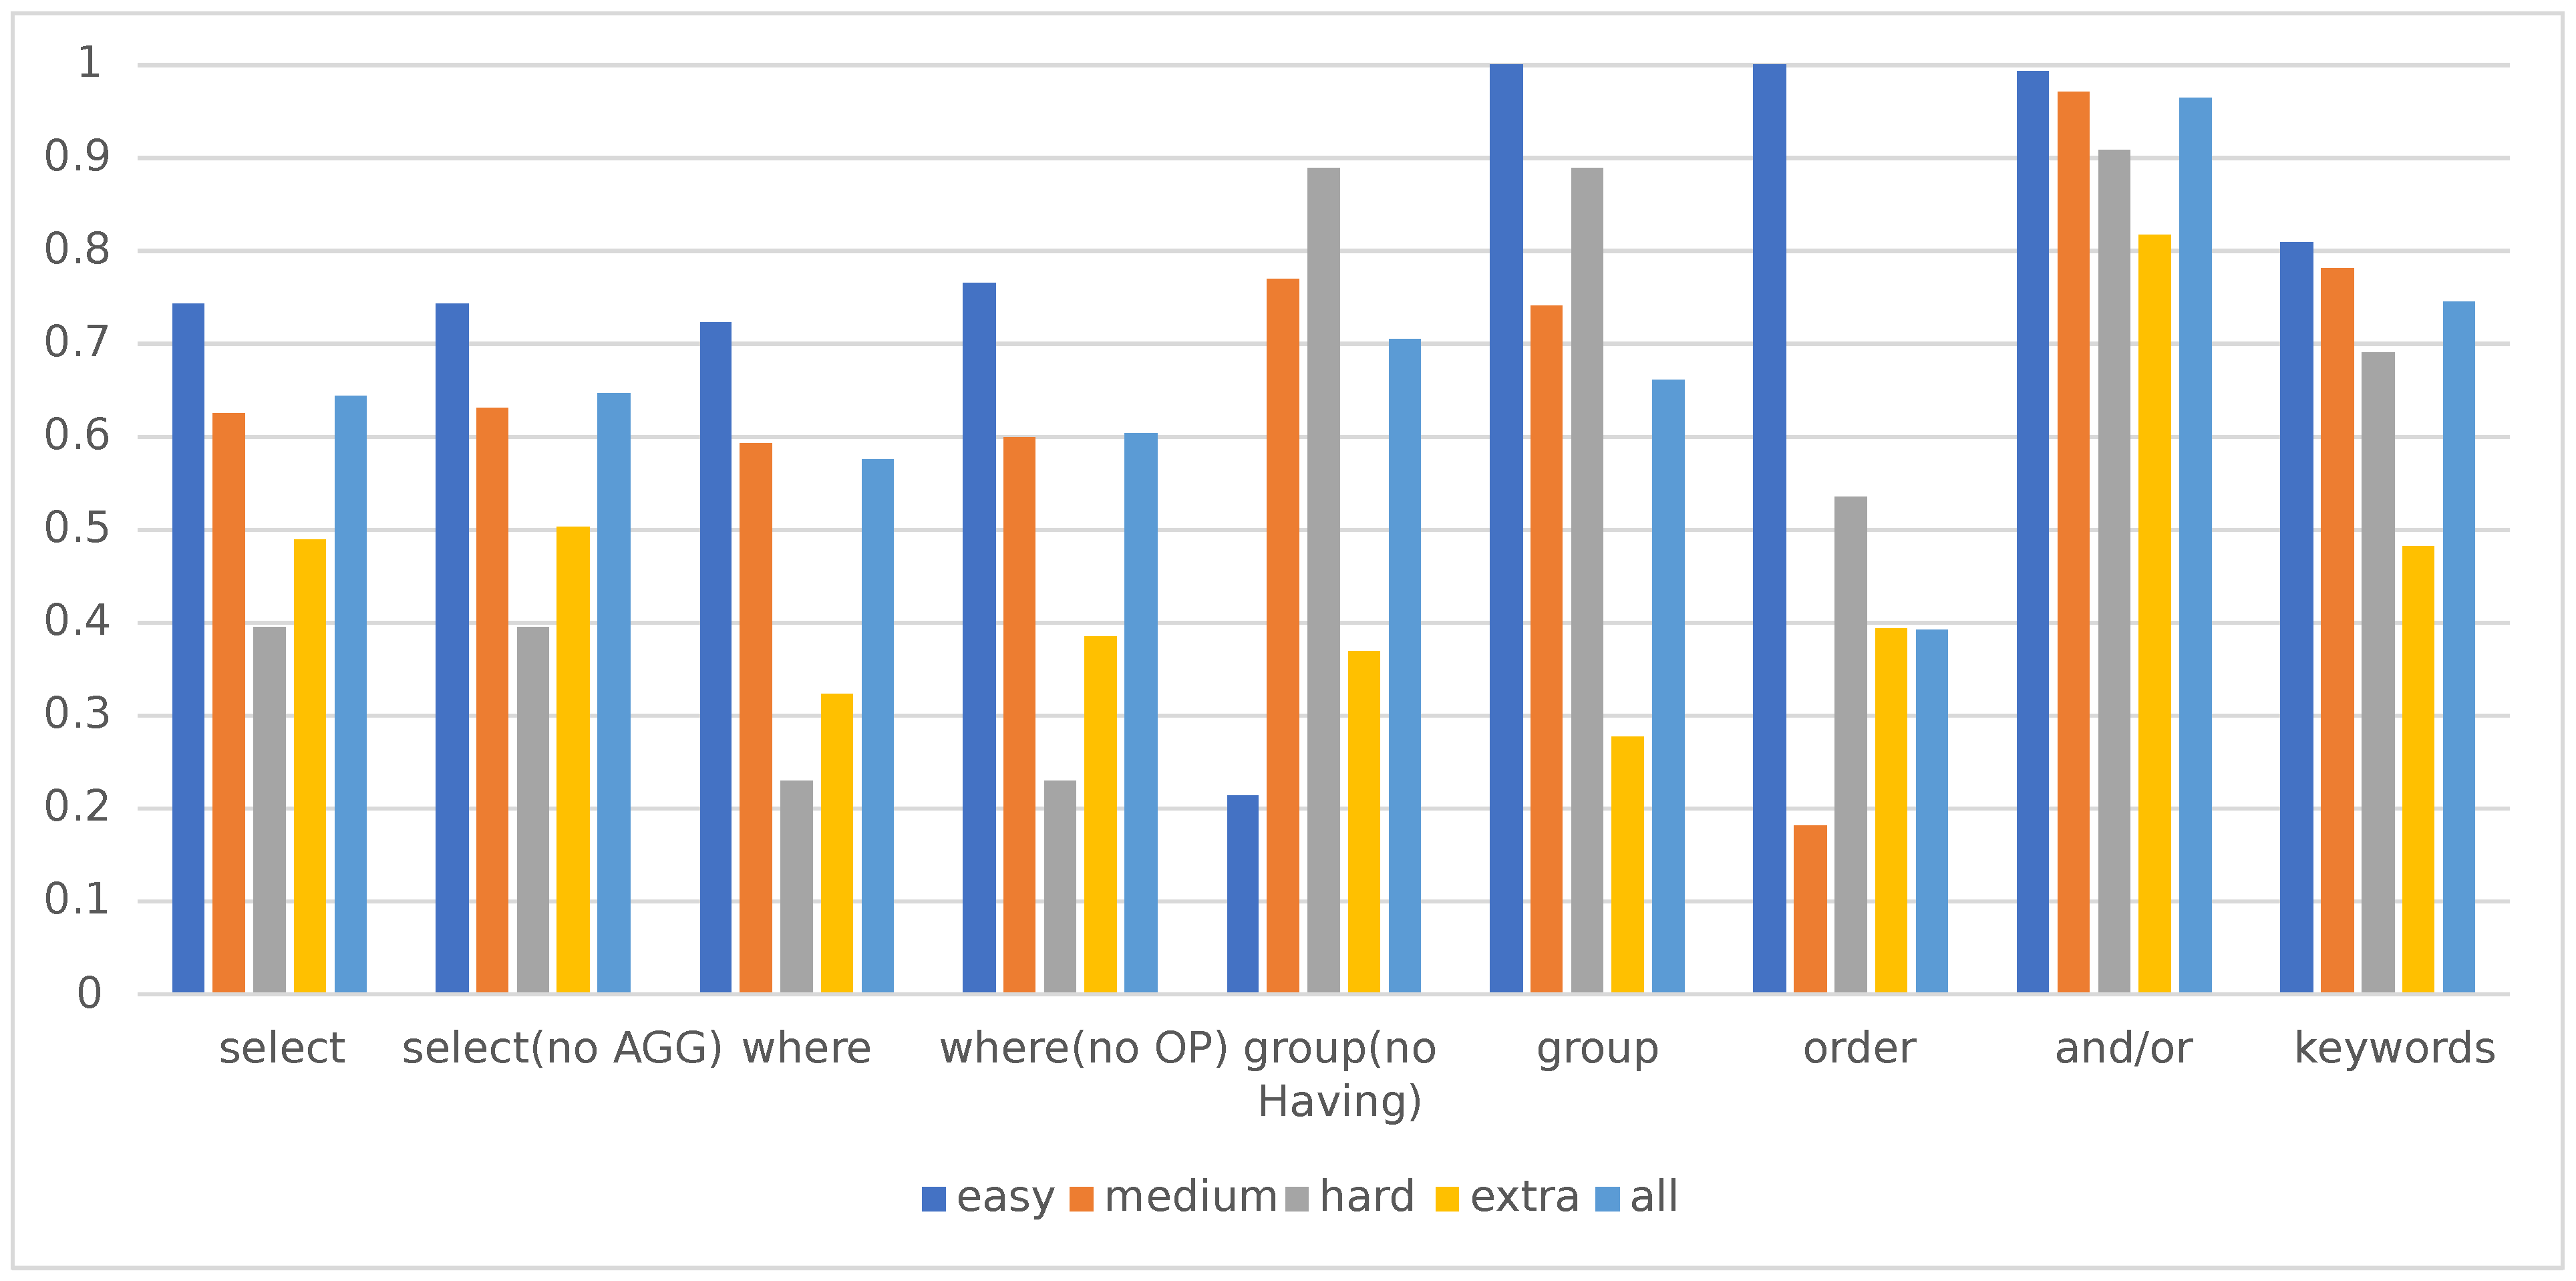
\includegraphics[width=1\textwidth]{pics/ez/F1eps}
    \caption{F1 Scores of Component Matching - PICARD T5-Large 4-Beam}
\end{figure}

Here, we can observe the F1 scores of each SQL Keyword for the PICARD T5-Large 4-Beam experiment on the SEOSS dataset. We can see that PICARD has managed to attain a very impressive F1 score for the SEOSS dataset without even having to be specifically trained for our dataset. This is a very encouraging result and indicates that the model is able to generalize accurately across different domains. Moreover, it is essential to note that the F1 score obtained by the PICARD model was obtained without any additional fine-tuning. This is a testament to the robustness and capability of the model and further highlights its ability to generalize to different datasets.

We experimented with a variety of different parameters, including beam size, modes and model sizes, and spent multiple hours for each evaluation. These experiments have been carefully documented in the Appendix of this thesis, where you can also find them in the project repository.

\subsection{EZ-PICARD - Microservices Practices}

% add image here
\begin{figure}[h]
    \centering
    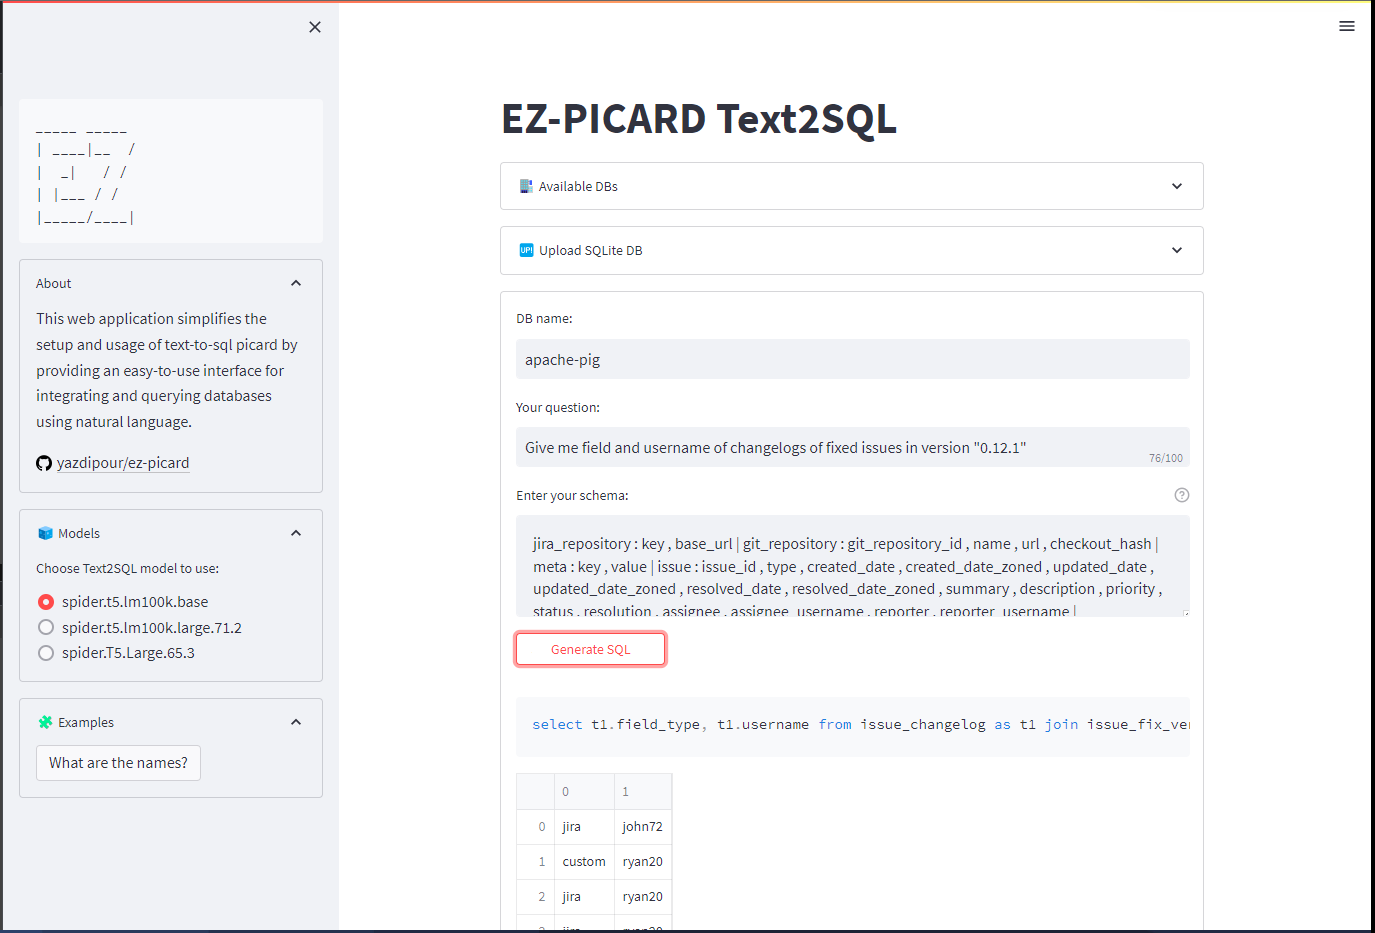
\includegraphics[width=1\textwidth]{pics/ez/ui.png}
    \caption{EZ-PICARD Web Application}
    \label{fig:ezpicard}
\end{figure}

For software engineering practices and to make PICARD setup easier for engineers, researchers, and users, a microservice web service with a web application has been created and open-sourced to the community\footnote[1]{Link to the Github Page: \url{https://github.com/yazdipour/ez-picard/}}. This application consists of a web user interface that gives users the ability to upload their databases and enter their natural language questions and receive queries from our model with values from the database if available. Additionally, a REST API exists for further expansion and usage within the application, providing users with a more versatile and powerful tool for their needs. This web service and application is designed to make the usage of PICARD easier and more accessible for everyone and to allow for the development of new applications and services that utilize its powerful capabilities.

PICARD is a method for constrained inference on top of an existing model, but it is not a model itself. Currently, the PICARD parser and the supporting software are not supported for PostgreSQL, MySQL and others, which would require changes to the PICARD parser, translation of Spider databases and text-to-SQL data, and retraining models to produce MSSQL code. To use the Picard Method, a complex toolchain of Haskell code is built with CABAL and requires a complicated toolchain for the Facebook Thrift library.

% After the setup, the Picard server can be started by running the compiled standalone executable PICARD. This executable is responsible for providing the necessary information to the user, such as specific parameters and options within the constrained inference.

The thrift library is used for communication between the parser and the beam search algorithm. The parser, written in the efficient and powerful Haskell programming language, is used in combination with the hf transformers, which is a Python package. To further expand the scope of the system, new SQL engines can be supported by adding a parser for each one.

These parsers also need to be written in Haskell, as the existing SQLite parser is of limited use in this regard, as it has been written to work best on Spider's subset of SQLite and only supports part of the SQLite specification. This means that more advanced parsers must be created to maximize the system's capabilities. Additionally, these parsers need to be written with a high level of precision in order to ensure that the system can effectively communicate with various engines and databases.

With EZ-PICARD, we can have an adapter layer between SQLite DB and any other database engine, such as MySQL. This layer can be implemented independently from PICARD itself using Python instead of Haskell and can provide a wide range of features, such as automatically translating queries from SQLite to the target database engine and mirroring the schema to the SQLite DB. This adapter layer can provide further advantages by allowing developers to use the same codebase to support multiple database engines, thus reducing the need for additional development and maintenance costs.

% add image here
\begin{figure}[h]
    \centering
    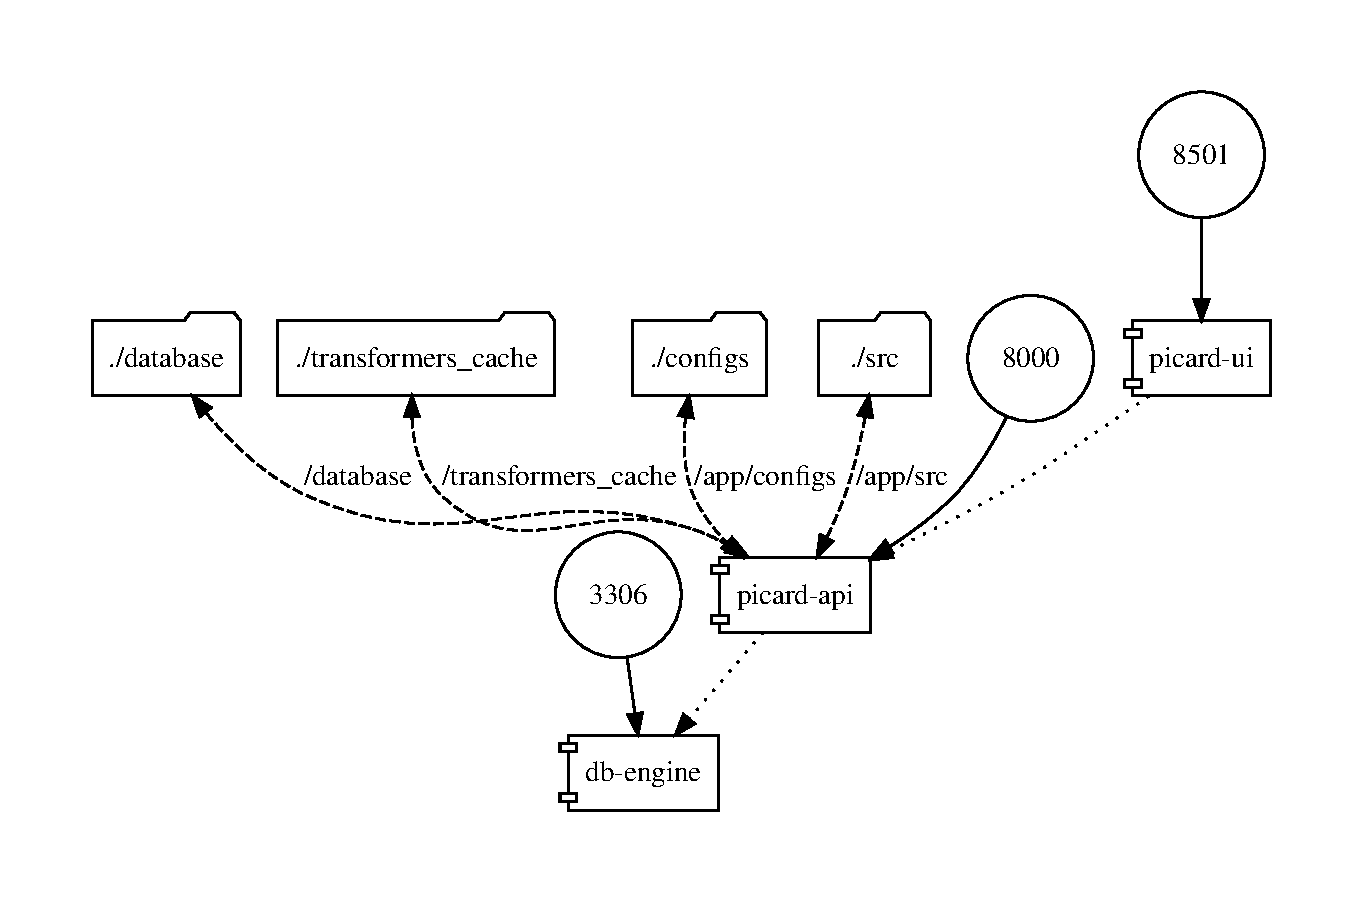
\includegraphics[width=0.8\textwidth]{pics/ez/mapeps}
    \caption{EZ-PICARD Architecture}
\end{figure}
\clearpage
\subsection{SEOSS evaluation with GPT 3.5 and GPT 4}  

Here we discuss our experience using the ChatGPT API for the Text-to-SQL task on the SEOSS dataset. We will provide a brief overview of the \ac{GPT} architecture and delve into the specifics of ChatGPT, emphasizing its capabilities and potential for addressing this particular challenge.
\subsubsection{GPT Architecture}

Generative Pre-trained Transformers (GPT) \cite{radford2018improving} represent the state-of-the-art in language modeling, being built upon the revolutionary Transformer architecture. This architecture has profoundly influenced the field of natural language processing due to its utilization of self-attention mechanisms. These mechanisms enable the parallel processing of sequences, leading to more efficient training and enhanced performance across a wide range of NLP tasks.

Inherently generative, GPT models are designed to create text based on the context they are given. They are pre-trained on vast quantities of textual data, which enables them to learn the underlying structure and patterns present in natural language. The pre-training phase consists of unsupervised learning using a masked language modeling objective. Following pre-training, GPT models can be fine-tuned for specific tasks, such as translation, summarization, or, as in our example, Text-to-SQL.

Prior to the introduction of GPT-4, OpenAI had developed three earlier GPT versions and had been refining GPT language models over an extended period. The first GPT model, launched in 2018, incorporated 117 million parameters. The next version, GPT-2, was released in 2019 and demonstrated a substantial increase, incorporating 1.5 billion parameters. GPT-3, which currently powers ChatGPT, made its debut in 2020 and operates with 175 billion parameters. OpenAI, however, has chosen not to reveal the number of parameters used in GPT-4 \cite{openai2023gpt4}.

Considering the consistent growth in parameter counts with each successive model, it is logical to assume that the most recent multimodal iteration features a higher number of parameters than its predecessor, GPT-3, which consists of 175 billion parameters. Also, some researchers have speculated that GPT-4 may have as many as 1 trillion parameters or more\cite{bubeck2023sparks}.

\subsubsection{ChatGPT}

\begin{figure}[H]
    \begin{AIbox}{Attention!}
        \parbox{1\textwidth}{
            Please note that the results in this section may be subject to change as ChatGPT continues to improve its system over time.
        }
    \end{AIbox}
\end{figure}


ChatGPT and \ac{LLM} models represent an evolution in language models tailored explicitly for conversational interfaces. These models exhibit a distinct behavior compared to older language models. While previous models operated on a text-in and text-out basis (accepting a prompt string and returning a completion to append to the prompt), GPT-3 and GPT-4 models follow a conversation-in and message-out approach \cite{bubeck2023sparks}. They expect input formatted in a chat-like transcript format and return a completion representing a model-generated message within the chat. This format is designed for multi-turn conversations but can also be effective in non-chat scenarios.
For our experiment with the SEOSS dataset, we utilized the ChatGPT API to submit natural language questions and retrieve generated SQL queries. The API allowed for the seamless integration of ChatGPT into our workflow and provided an efficient and effective means to process the dataset.
Throughout the evaluation, we observed that ChatGPT successfully generated accurate and syntactically correct SQL queries for a wide range of questions. The model excelled at handling complex queries and demonstrated a deep understanding of the underlying database schema.
However, there were instances where ChatGPT generated SQL queries that deviated from the desired output, particularly in edge cases and questions with ambiguous semantics. To mitigate this issue, we employed a combination of custom LLM prompts to ensure the generated queries met the required quality standards.

\subsubsection{ChatGPT Prompting}

\subsubsubsection{Rules}

ChatGPT employs prompts to direct its response generation process \cite{white2023prompt}. 
To maximize the effectiveness of ChatGPT in various applications, it is essential to understand the art of crafting effective prompts. The following guidelines have been established to optimize the performance of ChatGPT in generating accurate, relevant, and context-aware responses:

\begin{enumerate}
    \item \textbf{Give ChatGPT an identity and intended audience}: By assigning a role or identity to ChatGPT (e.g., "You are a text-to-sql assistant, do... or As an assistant, do...") and specifying the target audience, the model can adopt a specific perspective or tone, providing tailored responses to the context.

    \item \textbf{Offer and give specific context}: Including relevant background information or context in the prompt helps the model generate more accurate and meaningful answers, particularly when dealing with complex or domain-specific queries.

    \item \textbf{Highlight information to include or exclude}: Clearly specifying what information should be incorporated or omitted in the response enables ChatGPT to generate responses that better align with user expectations (e.g. "Do not use any aliases").

    \item \textbf{Choose a relevant tone of voice and writing style}: Indicating the desired tone (e.g., formal, informal) or writing style (e.g., persuasive, explanatory) in the prompt can guide ChatGPT in producing responses that are more suitable for the specific application.

    \item \textbf{Give examples to base the response on}: Providing example responses can help ChatGPT understand the desired output format and style, allowing it to generate similar responses.

    \item \textbf{Specify response length}: Mentioning the required response length (e.g., "In 256 characters or less, do...") helps in obtaining outputs that conform to the desired word count or character limit. When we know the desired response length, with this rule we can also control the number of tokens generated by the model that will have a cost effect.

    \item \textbf{Clarity and specificity}: Crafting clear and concise prompts, along with avoiding ambiguous or vague questions, can significantly improve the quality of the generated responses. Easily by providing exact information and clear instructions to the model, we can get significantly better results.
\end{enumerate}

These guidelines, when employed systematically, can enhance the performance of ChatGPT in a wide range of natural language processing tasks. By iterative refining and experimenting with different prompt styles, we can achieve improved outcomes in our specific applications.

\subsubsubsection{Roles}

Prompts are input messages with an associated role, which can fall into one of three categories: system, user, or assistant. The role of the message's author supplies context for the conversation and influences the model's response. \cite{openai2023gpt4}

\begin{itemize}
    \item \textbf{System}: A high-level directive for the conversation, typically used to offer guidance or establish the context for the assistant.
    \item \textbf{User}: A message submitted by the user, usually in the form of a question or a request for the assistant to process.
    \item \textbf{Assistant}: The response produced by the assistant is based on the context provided by the system and user messages. The assistant processes the messages according to their order in the list and generates a response accordingly. Employing system instructions can effectively guide the assistant's behavior throughout the conversation. The assistant prompt is usually used to provide historical context for the conversation. 
\end{itemize}

Now we outline our approach to discovering the optimal prompt for text-to-SQL ChatGPT agents and present some preliminary results.
The initial step in identifying the best prompt involves defining a set of criteria to evaluate the quality and accuracy of the generated SQL commands.

Potential criteria include the syntactic correctness of the SQL commands (i.e., adherence to the rules and patterns of SQL syntax) and the semantic correctness of the SQL commands (i.e., alignment with the meaning and intent of the natural language queries).

Given that ChatGPT is a conversational agent, we must also consider the quality of the output in terms of the context and format of SQL.
Consider an example from the SEOSS dataset: "Generate syntactically correct read-only SQL to answer the following question: What was changed in version 0.12.1." ChatGPT's output, in this case, would be a conversion with a query, which is not the desired outcome.

\begin{figure}[H]
    \begin{AIbox}{ChatGPT3.5-Turbo Prompt Attempt\#1}
        \vspace{-5px}
        \parbox{1\textwidth}{\scriptsize
        \begin{alltt} 
            {\bf Prompt:} \\ 
            Generate syntactically correct read-only SQL to answer the following question: What was changed in version 0.12.1
            \\
            {\bf ChatGPT:} \\
            Certainly! Here's the SQL statement to return what was changed in version 0.12.1:\\
            SELECT changes FROM version\_history WHERE version\_number = '0.12.1'. \\ Note that the syntax may vary slightly depending on the specific database management system being used and the structure of your tables,\\ but this should work in most cases assuming there is a table named version\_history with columns version\_number and changes.
        \end{alltt}
        }
        \vspace{-5px}
    \end{AIbox}
\end{figure}
%     \item \textbf{Goal}: \\\begin{lstlisting}
%     SELECT T1.field FROM issue_changelog AS T1 JOIN issue_fix_version AS T2 ON T1.issue_id = T2.issue_id WHERE T2.fix_version = "0.12.1"
% \end{lstlisting}

Now we must find a way to guide ChatGPT toward generating the correct SQL query. We can filter the result and obtain output in our desired style by specifying precisely what we want. The following is the prompt we used to enhance the quality of the output.

\begin{figure}[H]
    \begin{AIbox}{ChatGPT3.5-Turbo Prompt Attempt\#2}
        \vspace{-5px}
        \parbox{1\textwidth}{\scriptsize
        \begin{alltt} 
            {\bf Prompt:} \\ 
            Write one valid SQL query in markdown format without talking and giving a description. Generate syntactically correct read-only SQL to answer the following question: What was changed in version 0.12.1
            \\
            {\bf ChatGPT:} \\
            SELECT changes FROM version\_history WHERE version\_number = '0.12.1'
        \end{alltt}
        }
        \vspace{-5px}
    \end{AIbox}
\end{figure}

We can utilize the system role to provide context and the user role to pose the question. In the system role, we can limit the system to acting as an agent or assistant for a specific task. We can also supply the system with a database schema. We can present the question in the user role, and the assistant will generate the SQL query. We used the following prompt to improve the output quality as a text-to-SQL agent using the SEOSS dataset.

\begin{figure}[H]
    \begin{AIbox}{Final Prompt}
        \vspace{-5px}
        \parbox{1\textwidth}{\scriptsize
        \begin{alltt} 
            {\bf role(System):} \\ 
            You are a helpful assistant for generating syntactically correct read-only                   \\
            SQL to answer a given question.                                                              \\
            Database: \$dbname                                                                           \\
            The following are tables you can query:                                                      \\
            ---------------------                                                                        \\
            \$schemas                                                                                    \\
            ---------------------                                                                        \\
            Do not use IN keyword.                                                                       \\
            If it is necessary to use AS then use it like T1 T2 ..., but if the alias                    \\
            name is not going to be used in query again, then do not use.                                \\
            Do not filter WHERE for being NOT NULL if it is not necessary.                               \\
            If in using  COUNT(*) and COUNT(COLUMN) there is no difference then use COUNT(*). \\
            Write one valid SQL in markdown format.
            \\
            {\bf role(User):} \\
            Generate syntactically correct read-only SQL to answer the following question: \$question
        \end{alltt}
        }
        \vspace{-5px}
    \end{AIbox}
\end{figure}

% \begin{table}[h]
%     \centering
%     \begin{tabular}{|l|l|}
%         \hline
%         \textbf{Role} & \textbf{Content}                                                                             \\ \hline
%         System        & You are a helpful assistant for generating syntactically correct read-only                   \\
%                       & SQL to answer a given question.                                                              \\
%                       & Database: \$dbname                                                                           \\
%                       & The following are tables you can query:                                                      \\
%                       & ---------------------                                                                        \\
%                       & \$schemas                                                                                    \\
%                       & ---------------------                                                                        \\
%                       & Do not use IN keyword.                                                                       \\
%                       & If it is necessary to use AS then use it like T1 T2 ..., but if the alias                    \\
%                       & name is not going to be used in query again, then do not use.                                \\
%                       & Do not filter WHERE for being NOT NULL if it is not necessary.                               \\
%                       & \small{If in using $COUNT(*) and COUNT(COLUMN)$ there is no difference then use $COUNT(*)$.} \\
%                       & Write one valid SQL in markdown format.                                                      \\ \hline
%         User          & Generate syntactically correct read-only SQL to answer the following                         \\
%                       & question: \$question                                                                         \\ \hline
%     \end{tabular}
%     \caption{Prompt structure used in the Text-to-SQL task on the SEOSS dataset}
% \end{table}

By incorporating system and user roles, we effectively guide ChatGPT to generate the desired SQL query in response to a natural language question \cite{white2023prompt}. This approach demonstrates the importance of carefully crafting prompts and roles to achieve the most accurate and contextually appropriate results from ChatGPT in text-to-SQL tasks.

In this prompt, we first provided a system message that set the context for the system, including information about the database, tables, and specific syntax requirements for the generated SQL query. The user message then contained the natural language question for which the assistant was expected to generate the corresponding SQL query.
Using this prompt structure allowed us to effectively communicate the task requirements and constraints to ChatGPT, resulting in more accurate and syntactically correct SQL query generation.

Initially after generating queries and analyzing the results, we found that the generated SQL queries were syntactically correct but semantically incorrect or needed refinements. For instance, ChatGPT tent to use AS keyword to name tables even when It was not necessary or use IN keyword even for simple conditions. This sort of behavior tent to reduce the accuracy of the generated SQL queries and

\begin{table}[h]
    \centering
    \begin{tabular}{|l|l|}
        \hline
        \textbf{Prompt}         & \textbf{accuracy} \\ \hline
        Simple asking prompt    & 11\%              \\ \hline
        Prompt + Format constraints & 28\%              \\ \hline
        Prompt + Format Constraints + DB Schema         & 44\%              \\ \hline
    \end{tabular}
\end{table}

After running the GPT-3.5 model on the SEOSS dataset, we found that the accuracy of the generated SQL queries was 44.7\%. This is a significant improvement over the 11.6\% accuracy of the simple asking prompt. We also found that the accuracy of the generated SQL queries was 28.9\% when we added the format constraints to the prompt. This is a significant improvement over the 11\% accuracy of the simple asking prompt. We also found that the accuracy of the generated SQL queries was 44\% when we added the database schema to the prompt. This is a significant improvement over the 11\% accuracy of the simple asking prompt. After that, we did the same with GPT 4 and we saw a significant jump in accuracy, especially for easy and medium questions.

\begin{table}[h]
    \centering
    \begin{tabular}{|c|c|c|c|c|c|}
        \hline
        \multirow{2}*{Exact Match Accuracy} & easy  & medium & hard  & extra hard & all   \\
                                            & 392   & 378    & 77    & 84         & 931   \\ \hline
        SQLNet                              & 0.023 & 0.000  & 0.000 & 0.000      & 0.010 \\ \hline
        RatSQL + Glove                      & 0.309 & 0.214  & 0.091 & 0.000      & 0.224 \\ \hline
        RatSQL + Bert                       & 0.161 & 0.201  & 0.065 & 0.012      & 0.156 \\ \hline
        PICARD + T5Base + 4Beam             & 0.446 & 0.254  & 0.182 & 0.012      & 0.307 \\ \hline
        PICARD + T5Large + 4Beam            & 0.571 & 0.410  & 0.182 & 0.060      & 0.427 \\ \hline
        GPT 3.5-turbo                       & 0.551 & 0.460  & 0.130 & 0.190      & 0.447 \\ \hline
        GPT 4                               & 0.709 & 0.505  & 0.104 & 0.131      & 0.524 \\ \hline
    \end{tabular}
    \caption{Comparison between Exact Match Accuracy}
\end{table}

The table presents a comparison of the exact match accuracy for various models that have not been fine-tuned for our dataset. These models are assessed across five difficulty levels: easy, medium, hard, extra hard, and all. The large GPT models demonstrated the highest accuracy across all levels. Upon investigating the reasoning behind the lower accuracy on the hard level, we discovered that the model occasionally generated correct but complex queries, which led to confusion in our evaluation method.

\begin{table}[!ht]
    \centering
    \begin{tabular}{|c|c|c|L|L|}
        \hline
        Model                    & \textbf{Execution Accuracy} & \textbf{Time} & \textbf{Parameters}& \textbf{Cost}  \\ \hline
        PICARD + T5Base  & 0.307                       & ~400min       & 220M & Local Hardware \\ \hline
        PICARD + T5Large & 0.427                       & ~720min       & 770M & Local Hardware \\ \hline
        GPT 3.5-turbo            & 0.447                       & 37min         & 175B & \$2/iteration           \\ \hline
        GPT 4                    & 0.524                       & 78min         & 1T & \$14/iteration           \\ \hline
    \end{tabular}
    \caption{Expermiment Accuracy vs Resources used}
\end{table}
\subsection{Spider evaluation with GPT 3.5 and GPT 4}

Throughout this thesis, we have explored the advancements in Text-to-SQL models and their performance on the SPIDER benchmark. Our analysis revealed the significant progress made in the field, with more recent models demonstrating remarkable improvements in generating accurate SQL queries from natural language text.

The integration of powerful pre-trained language models, such as BERT, and cutting-edge architectures like T5 has played a vital role in the observed advancements. The models' ability to learn from limited labeled data, quickly adapt to new tasks or domains, and handle complex SQL queries has been substantially enhanced by employing techniques such as active learning, meta-learning, and multi-task learning.

Our experiments with ChatGPT-3.5 and ChatGPT-4.0 have showcased their superior performance, achieving scores of 81.30\% and 85.20\% on the SPIDER benchmark, respectively. These results highlight the potential of utilizing the latest huge language models for Text-to-SQL tasks, further pushing the boundaries of what is possible in this domain.

As the field of natural language processing continues to evolve, we can expect even more sophisticated models and techniques to emerge, enabling more accurate and efficient understanding and generation of SQL queries from natural language input. Future research in this area may focus on enhancing the models' ability to handle ambiguous or imprecise input, as well as exploring novel methods to improve their adaptability and generalization capabilities across diverse tasks and domains.

\begin{table}[h]
    \centering
    \begin{tabular}{|c|c|c|c|c|c|}
        \hline
        \multirow{2}*{Exact Match Accuracy} & easy  & medium & hard  & extra hard & all            \\
                                            & 248   & 446    & 174   & 166        & 1034           \\ \hline
        GPT 3.5 execution                   & 0.964 & 0.883  & 0.644 & 0.596      & 0.816          \\ \hline
        GPT 3.5 exact match                 & 0.972 & 0.881  & 0.621 & 0.596      & 0.813          \\ \hline
        GPT 4 execution                     & 0.980 & 0.930  & 0.678 & 0.651      & \textbf{0.855} \\ \hline
        GPT 4 exact match                   & 0.980 & 0.933  & 0.667 & 0.639      & \textbf{0.852} \\ \hline
    \end{tabular}
    \caption{Comparison between Exact Match Accuracy}
\end{table}

In conclusion, our experience using the ChatGPT API for the Text-to-SQL task on the SEOSS dataset was positive. The model's powerful natural language understanding capabilities, combined with the ease of integration through the API, make it a valuable tool for addressing such tasks. Additionally, by incorporating a few values from the database into the system input prompt, ChatGPT can better comprehend the database structure and generate more accurate queries. Also, by including the history of queries in prompts, we can improve the model's accuracy, but it will increase the overall time and money required to generate the queries. Future work could involve further fine-tuning ChatGPT specifically for Text-to-SQL tasks or exploring more advanced techniques for error correction and query validation.

% add SPIDER benchmark diagram image
\begin{figure}[h]
    \centering
    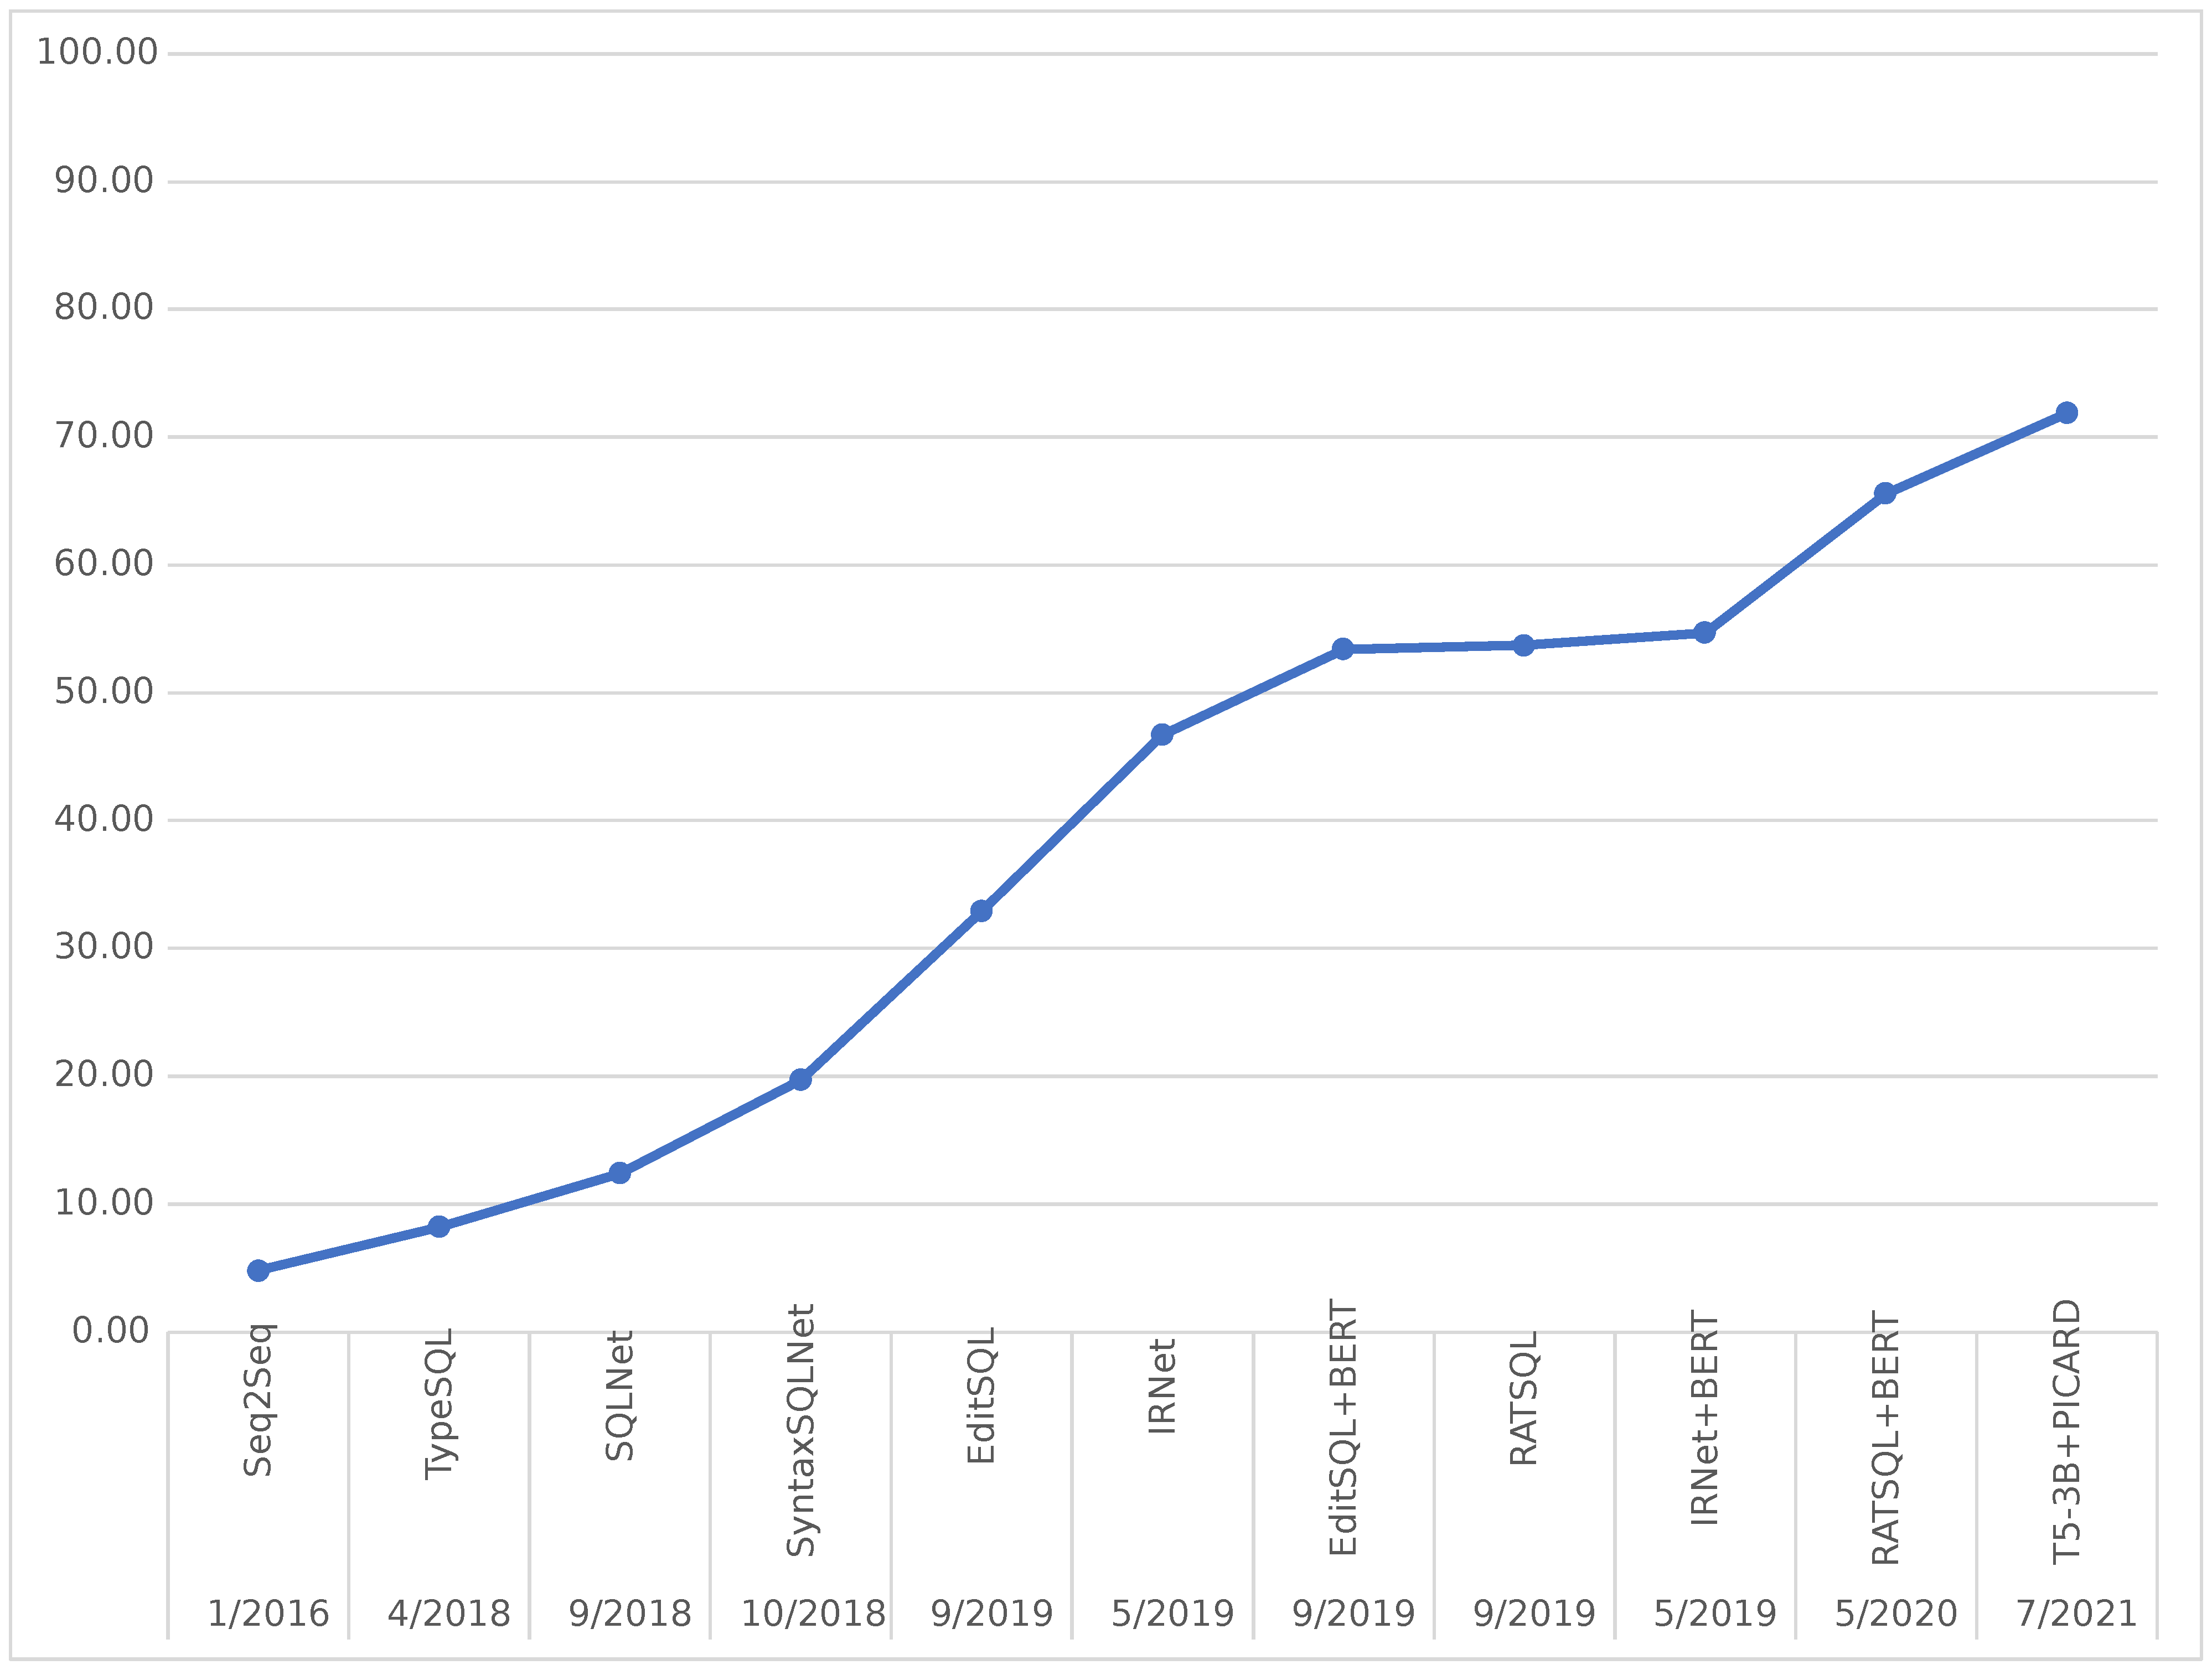
\includegraphics[width=0.99\linewidth]{pics/benchmarkeps}
    \caption{SPIDER benchmark Exact Match Results including our experiments}
    \label{fig:benchmark}
\end{figure}
\clearpage
\section{Conclusion and Future Directions}

This thesis provided a thorough analysis of state-of-the-art text-to-SQL solutions from a cross-domain perspective, offering a comprehensive overview of recent advancements in the field. We demonstrated the efficacy of pre-trained embeddings in enhancing schema linking and SQL structure accuracy through empirical results and aimed to elucidate the key similarities and differences between traditional and contemporary approaches.

An examination of the influence of datasets on text-to-SQL models' performance was carried out, with the Spider dataset and the demanding SEOSS dataset receiving special attention. Experiments with cutting-edge models, including ChatGPT, led us to identify the PICARD-T5 model as a promising option for further improvement through fine-tuning, provided that high-performance computing resources are accessible. These findings underscore the importance of considering model architecture and computational resources when evaluating NLP models.

Our study on evaluation metrics highlighted the need for more robust measures to assess text-to-SQL systems. Moreover, as research in the transformer and language models field expands, emerging challenges such as the Conversation-to-SQL task have surfaced, indicating areas requiring further exploration.

The text-to-SQL domain has seen significant progress recently, primarily due to the development of innovative datasets, models, and evaluation metrics. This field presents numerous opportunities for continued research and technological advancement, setting the stage for more advanced, efficient, and adaptable solutions to complex natural language processing tasks.

Moving forward, cross-domain text-to-SQL emerges as a promising area for further exploration. By incorporating domain-specific knowledge into models trained on existing datasets, models can become more adaptable across different domains, enhancing their capacity to handle scenarios with corrupted or unavailable tables. Real-world applications warrant attention, including advanced handling of user inputs not present in existing datasets and providing database administrators with tools to manage database schemas and update content.

The significant impact of Large Language Models (LLM) on various research fields, including text-to-SQL, suggests that their integration can lead to the development of more versatile question-answering systems for databases and dialogue systems with database-driven knowledge. Exploring the interconnection between SQL and other logical forms, as well as generalized semantic parsing, will contribute to a more comprehensive understanding of the subject, facilitating the creation of more adaptable and generalizable systems. Prompt learning, an emerging strategy within the LLM landscape, could enhance text-to-SQL systems' robustness by training models to respond to specific prompts or questions.

In conclusion, the text-to-SQL domain holds vast potential for growth and progress, with numerous practical applications and opportunities for integration with related fields, particularly in light of the ongoing advancements in large language models. The field's rapid growth signifies the importance of continual research into further advancements and improvements.


% \section{Conclusion}

% In this thesis, we provided an in-depth analysis of state-of-the-art text-to-SQL solutions from a cross-domain perspective, delivering a comprehensive overview of the latest advancements in the field. We demonstrated the efficacy of pre-trained embeddings in enhancing schema linking and SQL structure accuracy through empirical results. This study aimed to elucidate the fundamental similarities and differences between older models and contemporary approaches.

% We also examined datasets' influence on text-to-SQL models' performance, highlighting the Spider dataset as a challenging benchmark for text-to-SQL tasks and investigating the demanding SEOSS dataset. We conducted experiments with state-of-the-art models, including ChatGPT, and compared various models for text-to-SQL tasks. Our findings revealed that the PICARD-T5 model is a promising option, but further improvement could be achieved through fine-tuning, which might necessitate access to high-performance computing resources. These findings underscore the importance of considering both model architecture and computational resources when assessing the performance of NLP models.

% Our exploration of evaluation metrics emphasized the need for more robust measures to assess text-to-SQL systems. Additionally, as research in the transformer and language models field expands, emerging challenges such as the Conversation-to-SQL task have surfaced, indicating the need for further investigation.

% In conclusion, the text-to-SQL domain has experienced significant progress in recent years due to the creation of innovative datasets, models, and evaluation metrics. This area presents a wealth of opportunities for continued research and technological growth, paving the way for more advanced, efficient, and versatile solutions to complex natural language processing tasks.

% \clearpage
% \thispagestyle{plain}
% \section{Future Directions}

% The field of text-to-SQL is a rapidly growing area of research, encompassing numerous systems and approaches designed to generate SQL queries from natural language text. Despite considerable advancements, several areas still warrant further exploration and improvement.

% One promising direction for future research is cross-domain text-to-SQL. By incorporating domain-specific knowledge into models trained on existing datasets, these models can become more adaptable and applicable across different domains. This adaptability also enhances their capacity to handle scenarios where tables are corrupted or unavailable. Furthermore, addressing real-world applications, such as advanced handling of user inputs not present in existing datasets and providing database administrators with tools to manage database schemas and update content, is essential for the practical implementation of text-to-SQL systems. Multilingual text-to-SQL and developing database interfaces for individuals with disabilities are essential areas for future research.

% The growth of \ac{LLM} has significantly impacted various research fields, including text-to-SQL. Integrating text-to-SQL tasks into LLMs can lead to the development of more versatile question-answering systems for databases and dialogue systems with database-driven knowledge. Additionally, exploring the interconnection between SQL and other logical forms, as well as generalized semantic parsing, will contribute to a more comprehensive understanding of the subject, facilitating the creation of more adaptable and generalizable systems.
% Prompt learning, an emerging strategy within the LLM landscape, can be employed to enhance the robustness of text-to-SQL systems. This approach involves training models to respond to specific prompts or questions, thereby improving their performance in generating accurate SQL queries from natural language text.

% In conclusion, the domain of text-to-SQL holds immense potential for growth and progress, with numerous significant practical applications and opportunities for integration with related fields, particularly in light of the ongoing advancements in large language models.
\listoffigures
\addcontentsline{toc}{section}{List of Figures}

\listoftables
\addcontentsline{toc}{section}{List of Tables}

% -------------------- Bibliography --------------------
\renewcommand{\refname}{Bibliography}
\addcontentsline{toc}{section}{Bibliography}
\bibliographystyle{alpha}
\bibliography{bibs/litDB}

% -------------------- Appendix --------------------
% \clearpage
% \section*{Appendix}

\label{sec:appendix}

\begin{itemize}
    \item T5 base
    \item Mode: Lex
    \item maximum tokens to check: 2
    \item number of beams: 2
\end{itemize}

\begin{table}[h!]
    \centering
    \begin{tabular}{|c|c|c|c|c|c|}
        \hline
                 & easy  & medium & hard  & extra & all   \\ \hline
        select   & 0.873 & 0.624  & 0.469 & 0.500 & 0.717 \\ \hline
        where    & 0.882 & 0.824  & 0.308 & 0.421 & 0.780 \\ \hline
        group    & 0.000 & 0.805  & 0.969 & 0.556 & 0.726 \\ \hline
        order    & 0.000 & 0.409  & 0.469 & 0.400 & 0.431 \\ \hline
        and/or   & 1.000 & 0.929  & 0.896 & 0.598 & 0.927 \\ \hline
        keywords & 0.885 & 0.867  & 0.672 & 0.455 & 0.829 \\ \hline
    \end{tabular}
    \caption{PARTIAL MATCHING ACCURACY}
\end{table}

\begin{table}[h!]
    \centering
    \begin{tabular}{|c|c|c|c|c|c|}
        \hline
                 & easy  & medium & hard  & extra & all   \\ \hline
        select   & 0.597 & 0.373  & 0.390 & 0.131 & 0.447 \\ \hline
        where    & 0.756 & 0.429  & 0.229 & 0.104 & 0.477 \\ \hline
        group    & 0.000 & 0.520  & 0.886 & 0.119 & 0.490 \\ \hline
        order    & 0.000 & 0.321  & 0.429 & 0.095 & 0.267 \\ \hline
        and/or   & 0.992 & 1.000  & 0.986 & 0.961 & 0.993 \\ \hline
        keywords & 0.834 & 0.513  & 0.506 & 0.119 & 0.545 \\ \hline
    \end{tabular}
    \caption{PARTIAL MATCHING RECALL }

\end{table}
\begin{table}[h!]
    \centering
    \begin{tabular}{|c|c|c|c|c|c|}
        \hline
                 & easy  & medium & hard  & extra & all   \\ \hline
        select   & 0.709 & 0.467  & 0.426 & 0.208 & 0.551 \\ \hline
        where    & 0.814 & 0.564  & 0.262 & 0.167 & 0.592 \\ \hline
        group    & 1.000 & 0.632  & 0.925 & 0.196 & 0.585 \\ \hline
        order    & 1.000 & 0.360  & 0.448 & 0.154 & 0.329 \\ \hline
        and/or   & 0.996 & 0.963  & 0.939 & 0.737 & 0.959 \\ \hline
        keywords & 0.859 & 0.644  & 0.578 & 0.189 & 0.658 \\ \hline
    \end{tabular}
    \caption{PARTIAL MATCHING F1 }

\end{table}
\pagebreak

\begin{itemize}
    \item T5 base
    \item Mode: parse with guards
    \item maximum tokens to check: 2
    \item number of beams: 2
\end{itemize}

\begin{table}[h!]
    \centering
    \begin{tabular}{|c|c|c|c|c|c|}
        \hline
                 & easy  & medium & hard  & extra & all   \\ \hline
        select   & 0.873 & 0.624  & 0.469 & 0.500 & 0.717 \\ \hline
        where    & 0.882 & 0.824  & 0.308 & 0.421 & 0.780 \\ \hline
        group    & 0.000 & 0.805  & 0.969 & 0.556 & 0.726 \\ \hline
        order    & 0.000 & 0.409  & 0.469 & 0.400 & 0.431 \\ \hline
        and/or   & 1.000 & 0.929  & 0.896 & 0.598 & 0.927 \\ \hline
        keywords & 0.885 & 0.867  & 0.672 & 0.455 & 0.829 \\ \hline
    \end{tabular}
    \caption{PARTIAL MATCHING ACCURACY}
\end{table}

\begin{table}[h!]
    \centering
    \begin{tabular}{|c|c|c|c|c|c|}
        \hline
        select   & 0.597 & 0.373 & 0.390 & 0.131 & 0.447 \\ \hline
        where    & 0.756 & 0.429 & 0.229 & 0.104 & 0.477 \\ \hline
        group    & 0.000 & 0.520 & 0.886 & 0.119 & 0.490 \\ \hline
        order    & 0.000 & 0.321 & 0.429 & 0.095 & 0.267 \\ \hline
        and/or   & 0.992 & 1.000 & 0.986 & 0.961 & 0.993 \\ \hline
        keywords & 0.834 & 0.513 & 0.506 & 0.119 & 0.545 \\ \hline
    \end{tabular}
    \caption{PARTIAL MATCHING RECALL }

\end{table}
\begin{table}[h!]
    \centering
    \begin{tabular}{|c|c|c|c|c|c|}
        \hline
                 & easy  & medium & hard  & extra & all   \\ \hline
        select   & 0.709 & 0.467  & 0.426 & 0.208 & 0.551 \\ \hline
        where    & 0.814 & 0.564  & 0.262 & 0.167 & 0.592 \\ \hline
        group    & 1.000 & 0.632  & 0.925 & 0.196 & 0.585 \\ \hline
        order    & 1.000 & 0.360  & 0.448 & 0.154 & 0.329 \\ \hline
        and/or   & 0.996 & 0.963  & 0.939 & 0.737 & 0.959 \\ \hline
        keywords & 0.859 & 0.644  & 0.578 & 0.189 & 0.658 \\ \hline
    \end{tabular}
    \caption{PARTIAL MATCHING F1 }

\end{table}
\pagebreak
\begin{itemize}
    \item T5 base
    \item Mode: Lex
    \item maximum tokens to check: 2
    \item number of beams: 4
\end{itemize}

\begin{table}[h!]
    \centering
    \begin{tabular}{|c|c|c|c|c|c|}
        \hline
                 & easy  & medium & hard  & extra & all   \\ \hline
        select   & 0.858 & 0.623  & 0.483 & 0.571 & 0.713 \\ \hline
        where    & 0.863 & 0.804  & 0.333 & 0.474 & 0.771 \\ \hline
        group    & 0.000 & 0.812  & 0.968 & 0.500 & 0.699 \\ \hline
        order    & 0.000 & 0.391  & 0.484 & 0.444 & 0.431 \\ \hline
        and/or   & 1.000 & 0.921  & 0.870 & 0.602 & 0.921 \\ \hline
        keywords & 0.836 & 0.833  & 0.673 & 0.476 & 0.797 \\ \hline
    \end{tabular}
    \caption{PARTIAL MATCHING ACCURACY}

\end{table}
\begin{table}[h!]
    \centering
    \begin{tabular}{|c|c|c|c|c|c|}
        \hline
                 & easy  & medium & hard  & extra & all   \\ \hline
        select   & 0.538 & 0.341  & 0.377 & 0.143 & 0.409 \\ \hline
        where    & 0.714 & 0.418  & 0.229 & 0.117 & 0.460 \\ \hline
        group    & 0.000 & 0.469  & 0.857 & 0.095 & 0.448 \\ \hline
        order    & 0.000 & 0.321  & 0.429 & 0.095 & 0.267 \\ \hline
        and/or   & 0.995 & 1.000  & 0.971 & 0.980 & 0.994 \\ \hline
        keywords & 0.789 & 0.462  & 0.481 & 0.119 & 0.505 \\ \hline
    \end{tabular}
    \caption{PARTIAL MATCHING RECALL }

\end{table}

\begin{table}[h!]
    \centering
    \begin{tabular}{|c|c|c|c|c|c|}
        \hline
                 & easy  & medium & hard  & extra & all   \\ \hline
        select   & 0.661 & 0.441  & 0.423 & 0.229 & 0.520 \\ \hline
        where    & 0.782 & 0.550  & 0.271 & 0.188 & 0.576 \\ \hline
        group    & 1.000 & 0.594  & 0.909 & 0.160 & 0.546 \\ \hline
        order    & 1.000 & 0.353  & 0.455 & 0.157 & 0.329 \\ \hline
        and/or   & 0.997 & 0.959  & 0.918 & 0.746 & 0.956 \\ \hline
        keywords & 0.812 & 0.595  & 0.561 & 0.190 & 0.618 \\ \hline
    \end{tabular}
    \caption{PARTIAL MATCHING F1 }

\end{table}
\pagebreak
\begin{itemize}
    \item T5 base
    \item Mode: parse with guards
    \item maximum tokens to check: 2
    \item number of beams: 4
\end{itemize}

\begin{table}[h!]
    \centering
    \begin{tabular}{|c|c|c|c|c|c|}
        \hline
                 & easy  & medium & hard  & extra & all   \\ \hline
        select   & 0.757 & 0.537  & 0.417 & 0.469 & 0.618 \\ \hline
        where    & 0.779 & 0.746  & 0.250 & 0.433 & 0.695 \\ \hline
        group    & 0.000 & 0.658  & 0.971 & 0.391 & 0.561 \\ \hline
        order    & 0.000 & 0.269  & 0.457 & 0.526 & 0.407 \\ \hline
        and/or   & 1.000 & 0.910  & 0.883 & 0.619 & 0.919 \\ \hline
        keywords & 0.742 & 0.785  & 0.667 & 0.422 & 0.729 \\ \hline
    \end{tabular}
    \caption{PARTIAL MATCHING ACCURACY}

\end{table}
\begin{table}[h!]
    \centering
    \begin{tabular}{|c|c|c|c|c|c|}
        \hline
                 & easy  & medium & hard  & extra & all   \\ \hline
        select   & 0.653 & 0.442  & 0.390 & 0.274 & 0.511 \\ \hline
        where    & 0.690 & 0.464  & 0.171 & 0.169 & 0.475 \\ \hline
        group    & 0.000 & 0.571  & 0.971 & 0.214 & 0.552 \\ \hline
        order    & 0.000 & 0.250  & 0.457 & 0.238 & 0.314 \\ \hline
        and/or   & 0.992 & 0.997  & 1.000 & 1.000 & 0.995 \\ \hline
        keywords & 0.823 & 0.605  & 0.571 & 0.226 & 0.610 \\ \hline
    \end{tabular}
    \caption{PARTIAL MATCHING RECALL }

\end{table}
\begin{table}[h!]
    \centering
    \begin{tabular}{|c|c|c|c|c|c|}
        \hline
                 & easy  & medium & hard  & extra & all   \\ \hline
        select   & 0.701 & 0.485  & 0.403 & 0.346 & 0.560 \\ \hline
        where    & 0.732 & 0.572  & 0.203 & 0.243 & 0.564 \\ \hline
        group    & 1.000 & 0.612  & 0.971 & 0.277 & 0.556 \\ \hline
        order    & 1.000 & 0.259  & 0.457 & 0.328 & 0.355 \\ \hline
        and/or   & 0.996 & 0.951  & 0.938 & 0.765 & 0.956 \\ \hline
        keywords & 0.780 & 0.684  & 0.615 & 0.295 & 0.665 \\ \hline
    \end{tabular}
    \caption{PARTIAL MATCHING F1 }

\end{table}
\pagebreak
\begin{itemize}
    \item T5 large
    \item Mode: parse with guards
    \item maximum tokens to check: 2
    \item number of beams: 4
\end{itemize}

\begin{table}[h!]
    \centering
    \begin{tabular}{|c|c|c|c|c|c|}
        \hline
                 & easy  & medium & hard  & extra & all   \\ \hline
        select   & 0.781 & 0.672  & 0.400 & 0.552 & 0.684 \\ \hline
        where    & 0.739 & 0.689  & 0.269 & 0.396 & 0.642 \\ \hline
        group    & 0.000 & 0.756  & 0.865 & 0.391 & 0.675 \\ \hline
        order    & 0.000 & 0.250  & 0.528 & 0.542 & 0.462 \\ \hline
        and/or   & 1.000 & 0.947  & 0.831 & 0.699 & 0.937 \\ \hline
        keywords & 0.796 & 0.846  & 0.735 & 0.574 & 0.792 \\ \hline
    \end{tabular}
    \caption{PARTIAL MATCHING ACCURACY}
\end{table}

\begin{table}[h!]
    \centering
    \begin{tabular}{|c|c|c|c|c|c|}
        \hline
                 & easy  & medium & hard  & extra & all   \\ \hline
        select   & 0.709 & 0.585  & 0.390 & 0.440 & 0.608 \\ \hline
        where    & 0.708 & 0.520  & 0.200 & 0.273 & 0.523 \\ \hline
        group    & 0.000 & 0.726  & 0.914 & 0.214 & 0.649 \\ \hline
        order    & 0.000 & 0.143  & 0.543 & 0.310 & 0.343 \\ \hline
        and/or   & 0.987 & 0.997  & 1.000 & 0.983 & 0.992 \\ \hline
        keywords & 0.823 & 0.725  & 0.649 & 0.417 & 0.704 \\ \hline
    \end{tabular}
    \caption{PARTIAL MATCHING RECALL }

\end{table}

\begin{table}[h!]
    \centering
    \begin{tabular}{|c|c|c|c|c|c|}
        \hline
                 & easy  & medium & hard  & extra & all   \\ \hline
        select   & 0.743 & 0.625  & 0.395 & 0.490 & 0.644 \\ \hline
        where    & 0.723 & 0.593  & 0.230 & 0.323 & 0.576 \\ \hline
        group    & 1.000 & 0.741  & 0.889 & 0.277 & 0.661 \\ \hline
        order    & 1.000 & 0.182  & 0.535 & 0.394 & 0.393 \\ \hline
        and/or   & 0.994 & 0.971  & 0.908 & 0.817 & 0.964 \\ \hline
        keywords & 0.809 & 0.781  & 0.690 & 0.483 & 0.746 \\ \hline
    \end{tabular}
    \caption{PARTIAL MATCHING F1 }
\end{table}

\pagebreak
\begin{itemize}
    \item GPT
    \item Mode: 3.5 Turbo
\end{itemize}


\begin{table}[h!]
    \centering
    \begin{tabular}{|c|c|c|c|c|c|}
        \hline
                 & easy  & medium & hard  & extra & all   \\ \hline
        select   & 0.924 & 0.816  & 0.788 & 0.763 & 0.862 \\ \hline
        where    & 0.759 & 0.816  & 0.321 & 0.400 & 0.719 \\ \hline
        group    & 0.154 & 0.863  & 1.000 & 0.000 & 0.719 \\ \hline
        order    & 0.000 & 0.714  & 0.000 & 0.889 & 0.667 \\ \hline
        and/or   & 1.000 & 0.984  & 0.909 & 0.863 & 0.973 \\ \hline
        keywords & 0.868 & 0.911  & 0.469 & 0.543 & 0.838 \\ \hline
    \end{tabular}
    \caption{PARTIAL MATCHING ACCURACY}
\end{table}

\begin{table}[h!]
    \centering
    \begin{tabular}{|c|c|c|c|c|c|}
        \hline
                 & easy  & medium & hard  & extra & all   \\ \hline
        select   & 0.653 & 0.529  & 0.338 & 0.345 & 0.549 \\ \hline
        where    & 0.768 & 0.658  & 0.257 & 0.182 & 0.590 \\ \hline
        group    & 0.286 & 0.360  & 0.114 & 0.000 & 0.266 \\ \hline
        order    & 0.000 & 0.357  & 0.000 & 0.190 & 0.171 \\ \hline
        and/or   & 0.934 & 0.968  & 0.972 & 0.945 & 0.952 \\ \hline
        keywords & 0.903 & 0.574  & 0.195 & 0.226 & 0.573 \\ \hline
    \end{tabular}
    \caption{PARTIAL MATCHING RECALL }

\end{table}

\begin{table}[h!]
    \centering
    \begin{tabular}{|c|c|c|c|c|c|}
        \hline
                 & easy  & medium & hard  & extra & all   \\ \hline
        select   & 0.765 & 0.642  & 0.473 & 0.475 & 0.671 \\ \hline
        where    & 0.763 & 0.729  & 0.286 & 0.250 & 0.648 \\ \hline
        group    & 0.200 & 0.508  & 0.205 & 1.000 & 0.389 \\ \hline
        order    & 1.000 & 0.476  & 1.000 & 0.314 & 0.273 \\ \hline
        and/or   & 0.966 & 0.976  & 0.940 & 0.902 & 0.962 \\ \hline
        keywords & 0.885 & 0.704  & 0.275 & 0.319 & 0.680 \\ \hline
    \end{tabular}
    \caption{PARTIAL MATCHING F1 }
\end{table}
% \addcontentsline{toc}{section}{Appendix} % Add the appendix to the table of contents manually

\end{document}